%
% CHAPTER: Probability Theory
%

\chapterimage{Galton_box} % Chapter heading image

\chapter{Discrete Probability}
\label{chap:Probability Theory}

\begin{quote}
\begin{flushright}
\emph{The purpose of models is not to fit the data\\
but to sharpen the questions.}\\
Samuel Karlin
\end{flushright}
\end{quote}
\bigskip

Probability theory is the branch of mathematics that studies random experiments and phenomena. It assigns a numerical value to each possible outcome of an experiment, reflecting how likely that outcome is to occur. Even when the outcome of a specific experiment cannot be predicted in advance, probability theory allows us to analyze its properties and derive meaningful insights. For example, while we cannot foresee the next number drawn in a lottery, probability theory helps explain why spending all our savings on lottery tickets is an unwise strategy for becoming wealthy.

The significance of probability theory goes far beyond games of chance. It forms the mathematical foundation of statistical inference, allowing us to draw conclusions from data, and it underpins many machine learning algorithms used for classification and prediction with large datasets. Moreover, probability theory plays a vital role in fields such as finance, risk management, and the natural sciences, where understanding uncertainty and variability is crucial.

In this chapter, we focus on the area of discrete probability. In this version of the theory, the possible outcomes of an event are either finite or, at most, countably infinite. Our interest in discrete probability arises for two main reasons: first, due to its practical applications in learning from data; and second, because it has deep connections to several theoretical concepts explored in this book, such as the length of optimal codes, the probability that a random machine will halt, and the derivation of universal distributions based on Kolmogorov complexity. All of these connections are directly relevant to our theory of nescience.

We will cover only the most important concepts and results of probability theory. The material has been selected based on its relevance to the theory of nescience. For instance, moment-generating functions are not included. For a more comprehensive introduction to probability theory, refer to the references at the end of this chapter.

Our approach to probability theory will be formal and axiomatic. We will begin by stating a basic set of fundamental axioms, from which we will derive the main results and properties. Axioms are essential in mathematical theory, as they provide the foundation for constructing a consistent, universal, and rigorous framework. In the context of probability theory, they allow us to define and manipulate the elusive concept of probability in a way that is both precise and widely applicable.

%
% Section: Foundations of Probability Theory
%

\section{Interpretations of Probability}

The concept of \emph{probability} presents a profound intellectual challenge. Consider the case of rolling a die and computing the probability of obtaining an even number. The die has six distinct outcomes, and since half of them are even, we conclude that the probability is $3/6$, or equivalently $1/2$. This reflects the \emph{classical interpretation}\index{Classical interpretation of probability} of probability, which states that in an experiment where all finite outcomes are equally likely, the probability of an event is given by the ratio of favorable outcomes to the total number of possible outcomes.

However, this interpretation faces a problem of circularity: .the notion of "equally likely" often assumes a symmetry in the outcomes, but in formal contexts this can be criticized for relying implicitly on the very concept of probability it seeks to define. An alternative approach is the \emph{principle of indifference}\index{Principle of indifference}, which holds that in the absence of any relevant evidence, all outcomes should be assigned equal probability. This principle, however, breaks down when there is evidence suggesting that the outcomes are not equally probable. This principle, however, only applies in the absence of evidence. When information is available, such as knowing the die is loaded, it cannot be justifiably used, and the assumption of equally likely outcomes breaks down.

The \emph{frequentist interpretation}\index{Frequentist interpretation of probability} of probability posits that one should roll the die multiple times and compare the frequency of even outcomes to the total number of rolls. The fundamental idea is to repeat the experiment under similar conditions and assign to each outcome a probability equal to its relative frequency.

This interpretation, however, faces two major limitations. First, the notion of "similar conditions" is vague and lacks a precise definition; after all, if conditions were exactly identical in a deterministic system, the outcomes would also be identical. In practice, the assumption is that conditions are similar enough to allow statistical regularities to emerge. Second, the concept of a "large number of repetitions" is ill-defined—technically, the experiment must be repeated an infinite number of times.

From a practical standpoint, implementing the frequentist interpretation presents significant challenges. Some experiments, such as estimating the probability of a candidate winning an election, cannot be repeated. Moreover, probability is defined only in the context of a sequence of trials, which makes it impossible to compute the probability of a single, non-repeatable event. Finally, the interpretation assumes the existence of a limiting relative frequency, a condition that is not always satisfied, as illustrated by certain financial time series.

The \emph{subjective interpretation}\index{Subjective interpretation of probability}, representing a third approach to the concept of probability, proposes assigning probabilities to events based on our degree of belief: the stronger our conviction that an event will occur, the higher the probability we assign to it. However, not all possible probability assignments are acceptable; certain coherence conditions must be met. For example, assigning probabilities in a way that guarantees a loss in a betting system, a scenario known as a \emph{Dutch book}\index{Dutch book}, violates these conditions.

It turns out that the conditions necessary and sufficient to avoid such inconsistencies align precisely with the axioms of probability that will be introduced later. Thus, we are free to assign probabilities according to our beliefs, as long as these assignments remain consistent with those axioms.

A key limitation of the subjective interpretation is that degrees of belief can vary widely between individuals. The \emph{Bayesian interpretation}\index{Bayesian interpretation of probability} offers a refinement: we begin with an initial (prior) assignment of probabilities and update them as new evidence becomes available. As more evidence is accumulated, revised probabilities tend to converge to values that are more consistent with observed data, and under certain conditions, may approximate the long-run frequencies or objective probabilities (if such exist). Nevertheless, assigning probabilities to an infinite number of events is generally infeasible for humans.

Currently, the notion of probability is defined axiomatically through the \emph{axiomatic interpretation}\index{Axiomatic interpretation of probability}. This approach abandons the attempt to define probability explicitly, and instead accepts certain fundamental properties as given.

Mathematically, probability is defined as a real number between $0$ and $1$, where a probability of $0$ corresponds to an impossible event, and a probability of $1$ corresponds to an event that is certain to occur. Intuitively, however, we often express probabilities as percentages, for example, saying that it will rain tomorrow with a 70\% probability, which is also valid interpretation of the concept of probability.

Additional properties are also required. For example, if two events $A$ and $B$, with probabilities $P\left(A\right)$ and $P\left(B\right)$ respectively, are disjoint, then the probability of either $A$ or $B$ occurring should be $P\left(A\right) + P\left(B\right)$. If $A$ and $B$ can occur simultaneously and are independent (independence being a concept that is mathematically well-defined but often conceptually subtle), then the probability of both occurring together should be $P\left(A\right) P\left(B\right)$. Furthermore, the probability of $A$ occurring given that $B$ has already occurred should equal the fraction of the probability of $A$ that also lies within $B$.

%
% Section: Foundations of Probability Theory
%

\section{Foundations of Probability Theory}
\label{sec:probability_foundations}

Probability theory is fundamentally concerned with assigning numerical values to specific events drawn from a sample space \footnote{The term "event" in this context may seem somewhat counterintuitive, as it typically suggests that something has happened, an implication not always applicable in the mathematical setting. For example, consider the sample space of all possible outcomes from tossing a fair coin. A subset of this sample space might be the empty set, which represents no outcome at all. From a conventional perspective, this does not correspond to anything "happening," which may confuse readers unfamiliar with the mathematical usage of the term. Nevertheless, for consistency and clarity, we will continue to use the term "events" to refer to subsets of the sample space.}.

\begin{definition}
Given $\left( \Omega, \mathcal{A} \right)$ as a field over a non-empty discrete set, $\Omega$ is called the \emph{sample space}\index{Sample space}, its elements are called \emph{outcomes}\index{Outcome}, and the elements of $\mathcal{A}$ are referred to as \emph{events}\index{Event}. Specifically, $\Omega$ is known as the \emph{certain event}\index{Certain event}, while the empty set $\varnothing$ is called the \emph{impossible event}\index{Impossible event}.
\end{definition}

As discussed in Section \ref{sec:sets}, since $\left( \Omega, \mathcal{A} \right)$ is a field, it follows that $\Omega \in \mathcal{A}$ and $\varnothing \in \mathcal{A}$. Moreover, the union of a finite collection of events is also an event: $A_1 \cup A_2 \cup \ldots \cup A_n \in \mathcal{A}$, and likewise, the intersection of a finite collection of events is an event: $A_1 \cap A_2 \cap \ldots \cap A_n \in \mathcal{A}$.

As mentioned in the introduction to this chapter, our primary focus is on discrete mathematics. Accordingly, we will concentrate on probabilities defined over discrete sets, whether finite or countably infinite. Extending the concept of probability to continuous sets requires the use of $\sigma$-algebras\index{$\sigma$-algebra} of sets instead of fields, along with the tools of measure theory. On a philosophical level, one might argue that all sample spaces must be countable, since physical measurements cannot be made with infinite precision. In practice, this is indeed the case: any empirical observation is subject to finite resolution.

The standard axiomatization used in probability theory is encapsulated in the framework of the \emph{Kolmogorov axioms}\footnote{In discrete probability theory, the sample space consists of a finite or countably infinite set of distinct outcomes. As a result, events are typically made up of individual, separable outcomes. Since probabilities are assigned directly to these discrete events, only finite unions of disjoint events need to be considered in Axiom 3 to account for all practical cases.}.

\begin{definition} (\emph{Kolmogorov's Axioms})\index{Kolmogorov's axioms}\label{Kolmogorov_axioms}
A \emph{probability}\index{Probability} is a real number $P(A) \in \mathbb{R}$ assigned to each event $A \in \mathcal{A}$ in the field $\left( \Omega, \mathcal{A} \right)$, subject to the following axioms:

\medskip

\begin{description}
\item [Axiom 1] Non-negativity: For all events $A \in \mathcal{A}$, we have $P(A) \geq 0$.
\item [Axiom 2] Normalization: The probability of the certain event is one, i.e., $P(\Omega) = 1$.
\item [Axiom 3] Additivity: For any finite sequence of pairwise disjoint events $A_1, A_2, \ldots, A_n \in \mathcal{A}$, the probability of their union equals the sum of their individual probabilities:
\[
P\left(\bigcup_{i=1}^n A_i\right) = \sum_{i=1}^n P(A_i).
\]
\end{description}

The triplet $\left( \Omega, \mathcal{A}, P \right)$ is called a \emph{probability space}\index{Probability space}.
\end{definition}

Despite their foundational importance, the Kolmogorov axioms present certain limitations. While they establish essential constraints on any probability function (such as non-negativity, normalization, and additivity) they do not prescribe how to assign probabilities to specific events. In other words, the axioms define the formal rules that probabilities must satisfy but remain silent on how those probabilities should be determined in practice. This is a consequence of their high level of generality: any mathematical structure that satisfies these properties can be regarded as a valid probability model. As such, they are abstract enough to encompass not only probability measures but also other normalized physical measures such as mass, volume, or charge.

From an intuitive standpoint, it might seem more natural to assign probabilities directly to the individual elements of the sample space, especially in the discrete case where each outcome is well, defined and countable. However, in the formal theory of probability, probabilities are assigned to events, which are subsets of the sample space. This approach, though less intuitive at first glance, ensures compatibility with the measure-theoretic framework that underlies modern probability theory. In the continuous case, individual outcomes (such as a specific real number) typically have probability zero, and probability must be defined directly over sets (e.g., intervals) rather than points.

\begin{example}
\label{ex:discrete_sample_space}
Consider a sample space $\Omega$ consisting of $n$ equally probable outcomes. If an event $A \subset \Omega$ contains $d(A) = m$ elements, then the probability of event $A$ is given by $P(A) = m/n$.
\end{example}

We now proceed to establish some fundamental results in probability theory, beginning with the calculation of the probability of the complement of an event, that is, the probability that the event does not occur.

\begin{proposition}
For any event $A$, it holds that $P\left( A^{c} \right) = 1 - P\left( A \right)$.
\end{proposition}

\begin{proof}
The sets $A$ and $A^c$ are disjoint, and their union satisfies $A \cup A^c = \Omega$. By Axiom 3 (additivity), we have $
P\left( A \cup A^c \right) = P\left( A \right) + P\left( A^c \right)$. By Axiom 2 (normalization), we know that $P\left( A \cup A^c \right) = P(\Omega) = 1$. Combining both equations, we obtain $P\left( A \right) + P\left( A^c \right) = 1,
$ which completes the proof.
\end{proof}

As a direct consequence of the previous proposition, we can deduce the probability of the impossible event.

\begin{proposition}
The probability of the impossible event is zero; that is, $P\left( \varnothing \right) = 0$.
\end{proposition}
\begin{proof}
Since $\varnothing = \Omega^c$, we apply the complement rule:
\[
P\left( \varnothing \right) = P\left( \Omega^c \right) = 1 - P\left( \Omega \right) = 1 - 1 = 0.
\]
\end{proof}

As expected, sub-events (i.e., subsets) are associated with probabilities no greater than those of the events containing them.

\begin{proposition}
If $A \subset B$, then $P\left( A \right) \leq P\left( B \right)$.
\end{proposition}
\begin{proof}
The event $B$ can be written as the disjoint union of $A$ and $B \cap A^c$. By Axiom 3: $P\left( B \right) = P\left( A \right) + P\left( B \cap A^c \right)$. Since $P\left( B \cap A^c \right) \geq 0$, it follows that $P\left( A \right) \leq P\left( B \right)$.
\end{proof}

With these basic properties established, we can now confirm that all probabilities lie between zero and one.

\begin{proposition}
For any event $A$, we have $0 \leq P\left( A \right) \leq 1$.
\end{proposition}
\begin{proof}
By Axiom 1, $P\left( A \right) \geq 0$. Since $A \subset \Omega$, the previous proposition implies $P\left( A \right) \leq P\left( \Omega \right) = 1$.
\end{proof}

Axiom 3 allows us to compute the probability of the union of disjoint events. However, it does not directly apply to cases involving non-disjoint events. The following proposition provides a formula for computing the probability of the union of two events that may overlap.

\begin{proposition}
For any two events $A$ and $B$, we have:
\[
P\left(A \cup B\right) = P\left(A\right) + P\left(B\right) - P\left(A \cap B\right).
\]
\end{proposition}

\begin{proof}
The union of $A$ and $B$ can be expressed as $A \cup B = \left( A \setminus B \right) \cup B$. Since $A \setminus B$ and $B$ are disjoint, by Axiom 3 we obtain:
\[
P\left( A \cup B \right) = P\left( B \right) + P\left( A \setminus B \right).
\]
Now, observe that $P\left( A \right) = P\left( A \setminus B \right) + P\left( A \cap B \right)$, which implies:
\[
P\left( A \setminus B \right) = P\left( A \right) - P\left( A \cap B \right).
\]
Substituting this into the previous expression yields:
\[
P\left( A \cup B \right) = P\left( B \right) + P\left( A \right) - P\left( A \cap B \right),
\]
as required.
\end{proof}

This result generalizes to any finite number of events via the \emph{principle of inclusion-exclusion}\index{Inclusion-exclusion principle} (see Section \ref{sec:counting}):
\begin{equation*}
\begin{split}
P \left( \bigcup_{i=1}^n A_i \right) & = \sum_{i=1}^n P \left( A_i \right) - \sum_{i<j} P \left( A_i \cap A_j \right) + \sum_{i<j<k} P \left( A_i \cap A_j \cap A_k \right) - \\
& \sum_{i<j<k<l} P \left( A_i \cap A_j \cap A_k \cap A_l \right) + \ldots +  (-1)^{n+1} P \left( A_1 \cap \ldots \cap A_n \right)
\end{split}
\end{equation*}

To ensure that a probability function satisfies Kolmogorov's axioms, we must define it using methods that are guaranteed to produce valid probability measures. One such method involves assigning probabilities to individual elements of a finite or countable sample space and extending this assignment to subsets via summation.

\begin{proposition}
Let $\left( \Omega, \mathcal{A} \right)$ be a field over a non-empty discrete set, and let $p_1, p_2, \ldots$ be a sequence of nonnegative real numbers such that $\sum_{i=1}^\infty p_i = 1$. Define a function $P : \mathcal{A} \to [0,1]$ by $P(A) = \sum_{\{ i : s_i \in A \}} p_i$, with the convention that the sum over an empty index set is 0. Then $P$ is a probability on $\left( \Omega, \mathcal{A} \right)$.
\end{proposition}
\begin{proof}
We must verify that the function $P$ satisfies the three Kolmogorov axioms:

Axiom 1 (Nonnegativity): Let $A \in \mathcal{B}$. Since each $p_i \geq 0$, the sum
\[
P(A) = \sum_{\{ i : s_i \in A \}} p_i
\]
is a (possibly infinite) sum of nonnegative terms. Hence, $P(A) \geq 0$.

Axiom 2 (Normalization): We have that
\[
P(\Omega) = \sum_{\{ i : s_i \in \Omega \}} p_i = \sum_{i=1}^\infty p_i = 1,
\]
by assumption. Hence, $P(\Omega) = 1$.

Axiom 3 (Finite Additivity): Let $A_1, \ldots, A_n \in \mathcal{B}$ be pairwise disjoint events. Define $A = \bigcup_{j=1}^n A_j$. Then the sets $\{ i : s_i \in A_j \}$ are disjoint for distinct $j$, and we have:
\[
P(A) = \sum_{\{ i : s_i \in A \}} p_i = \sum_{j=1}^n \sum_{\{ i : s_i \in A_j \}} p_i = \sum_{j=1}^n P(A_j),
\]
where we used the disjointness of the $A_j$'s and associativity of finite sums.

Hence, $P$ satisfies all three axioms of probability (with finite additivity), and is therefore a valid probability function on $\left( \Omega, \mathcal{A} \right)$.
\end{proof}

Finally, we introduce the concept of a probability mass function\footnote{Most probability textbooks define the probability mass function as a real-valued function of the form $f : \mathbb{R} \rightarrow [0, 1]$. However, this definition requires the prior introduction of the concept of a random variable. Since random variables play a more secondary role in the context of discrete probability, we have postponed their introduction to a later subsection. For this reason, we have provided a definition of the probability mass function based directly on events.
}. A probability mass function assigns a probability to each event in a discrete sample space.

\begin{definition}
\label{def:probability_function}
Let $\left( \Omega, \mathcal{A}, P \right)$ be a discrete probability space. A \emph{probability mass function}\index{Probability mass function} is a real-valued function $f : \mathcal{A} \rightarrow [0, 1]$ such that $f(A) = P(A)$ for every $A \in \mathcal{A}$.
\end{definition}

In Example \ref{ex:discrete_sample_space}, we introduced a discrete probability space $\left( \Omega, \mathcal{A}, P \right)$ consisting of $n$ equally probable elements. The corresponding probability mass function is defined as $f : \mathcal{A} \rightarrow [0, 1]$, with
\[
f(A) = \frac{d(A)}{n}, \quad \text{for all } A \in \mathcal{A},
\]
where $d(A)$ denotes the number of elements in the event $A$.

In many discrete settings, it is common to treat each individual element $\omega \in \Omega$ as an elementary event. That is, we assume that every set $\{\omega\}$ belongs to $\mathcal{A}$. In this case, we can define the probability mass function as a function $f : \Omega \rightarrow [0,1]$, where $f(\omega) = P(\{\omega\})$ for each $\omega \in \Omega$. This formulation is often more natural, as it allows us to specify probabilities at the level of individual outcomes.

The following proposition shows that, under this assumption, the probability of any event $A \in \mathcal{A}$ can be computed by summing the probabilities of the individual outcomes that make up the event.

\begin{proposition}
Let $\left( \Omega, \mathcal{A}, P \right)$ be a discrete probability space such that $\{\omega\} \in \mathcal{A}$ for every $\omega \in \Omega$. Define the function $f : \Omega \rightarrow [0,1]$ by $f(\omega) = P(\{\omega\})$. Then for any event $A \in \mathcal{A}$, the probability of $A$ is given by:
\[
P(A) = \sum_{\omega \in A} f(\omega).
\]
\end{proposition}
\begin{proof}
Since $A \in \mathcal{A}$, and $\{\omega\} \in \mathcal{A}$ for each $\omega \in \Omega$, it follows that every singleton $\{\omega\} \subseteq A$ is a measurable event. Furthermore, the singletons $\{ \omega \}$ for $\omega \in A$ are pairwise disjoint and their union is exactly $A$. Thus, by Axiom 3 (finite additivity),
\[
P(A) = P\left( \bigcup_{\omega \in A} \{\omega\} \right) = \sum_{\omega \in A} P(\{\omega\}) = \sum_{\omega \in A} f(\omega).
\]
\end{proof}

%
% Section: Conditional Probability
%

\section{Conditional Probability}
\label{sec:probability_conditional}

The concept of conditional probability plays a fundamental role in statistical learning. Conditional probability allows us to refine the probability of an event based on new information or imposed conditions. Within the axiomatic framework established by Kolmogorov, conditional probability is introduced as a definition.

\begin{definition}
Let $A$ and $B$ be two events such that $P(B) > 0$. The \emph{conditional probability}\index{Conditional probability} of $A$ given $B$, denoted by $P(A \mid B)$, is defined as:
\[
P(A \mid B) = \frac{P(A \cap B)}{P(B)}.
\]
\end{definition}

Because it satisfies the Kolmogorov axioms, a conditional probability is itself a valid probability. Note that $P(A \mid B)$ is undefined when $P(B) = 0$.

Some scholars argue that, given its central role in probability theory, conditional probability should be a property logically deduced from the foundational axioms, rather than introduced as a definition. This viewpoint naturally calls for an extension of Definition \ref{Kolmogorov_axioms}\index{Kolmogorov's axioms} to include additional properties. Unfortunately, there is no consensus among mathematicians or philosophers on how such an extension should be formalized.

The standard interpretation of conditional probability views it as the updated probability of event $A$ given that event $B$ has occurred. This interpretation, however, may implicitly suggest a temporal or even causal relationship between $B$ and $A$, a suggestion that is not necessarily valid.

\begin{example}
\label{ex:concurrent_events}
Suppose we are playing a game with a standard deck of 52 cards and we draw two cards. Let event $A$ be “drawing at least one heart,” and event $B$ be “drawing at least one queen.” These two events are dependent, as the occurrence of $B$ affects the probability of $A$. However, the events are not temporally related, since both cards are drawn simultaneously, one does not occur before the other. This example illustrates that dependency in probability theory does not require a temporal sequence between the events involved.
\end{example}

The probability of two events occurring together (though not necessarily in a temporal sequence, as discussed in Example \ref{ex:concurrent_events}), given their conditional relationship, is captured by the formula $P \left( A \cap B \right) = P \left( A \mid B \right) P \left( B \right)$. This equation often provides a more intuitive understanding of the concept of conditional probability. In fact, several authors have argued that this formulation should serve as the primary definition of conditional probability, rather than the quotient-based approach.

This formula generalizes to any finite number of events through what is known as the \emph{multiplication rule}\index{Multiplication rule}, which is expressed as:
\begin{equation}\label{eq:multiplication_rule}
P \left( A_{1} \cap A_{2} \cap \ldots \cap A_{n} \right) = P \left( A_{1} \right) P \left( A_{2} \mid A_{1}\right) \ldots  P \left( A_{n} \mid A_{1}\cap A_{2} \cap \ldots \cap A_{n-1} \right)
\end{equation}

The concept of event independence plays a central role in probability theory and statistical learning.

\begin{definition}\label{independent_events}\index{Independent events}
Two events $A$ and $B$ are declared to be \emph{independent} if $P \left( A \cap B \right) = P \left( A \right) P \left(B \right)$.
\end{definition}

Intuitively, events $A$ and $B$ are considered independent if knowing that event $B$ has occurred does not affect the probability of event $A$. This property follows logically from the definition of independence.

\begin{proposition}
Let $A$ and $B$ be two events such that $P \left( A \right) > 0$ and $P \left( B \right) > 0$. Then $A$ and $B$ are independent if and only if $P \left( A \mid B \right) = P \left( A \right)$.
\end{proposition}
\begin{proof}
Assume $A$ and $B$ are independent, i.e., $P \left( A \cap B \right) = P \left( A \right) P \left( B \right)$. Then,
\[
P \left( A \mid B \right) = \frac{P \left( A \cap B \right)}{P \left( B \right)} = \frac{P \left( A \right) P \left( B \right)}{P \left( B \right)} = P \left( A \right).
\]
Conversely, assume that $P \left( A \mid B \right) = P \left( A \right)$. Then by the multiplication rule,
\[
P \left( A \cap B \right) = P \left( A \mid B \right) P \left( B \right) = P \left( A \right) P \left( B \right),
\]
which confirms independence.
\end{proof}

Note that if $P \left( A \mid B \right) = P \left( A \right)$, then it also follows that $P \left( B \mid A \right) = P \left( B \right)$. This is a direct consequence of the fact that the joint probability $P \left( A \cap B \right)$ can be expressed as $P \left( A \right) P \left( B \right)$.

As in the case of conditional probability, some scholars have argued that independence should not be treated merely as a definition, but rather as a logical consequence of the foundational axioms of probability. However, incorporating independence as a derived property would require extending or modifying the axiomatic system, a topic for which no universally accepted approach currently exists.

The concept of independence can be generalized to collections of more than two events. The events $A_{1}, \ldots, A_{n}$ are said to be \emph{mutually independent}\index{Mutually independent events} if, for every subset of events $A_{i_1}, \ldots, A_{i_j}$ with $j \in {2, 3, \ldots, n}$, the following condition holds:
\[
P \left( A_{i_1} \cap \ldots \cap A_{i_j} \right) = P \left( A_{i_1} \right) \cdots P \left( A_{i_j} \right).
\]
It is important to emphasize that \emph{pairwise independence}\index{Pairwise independent events}, that is, the condition $P(A_i \cap A_j) = P(A_i)P(A_j)$ for all $i \neq j$, is not sufficient to guarantee mutual independence. Mutual independence requires that the product rule holds for \emph{every} subset of two or more events, not just for pairs.

\begin{example}
Confusion often arises when distinguishing between mutually exclusive (or disjoint) events and independent events. For two mutually exclusive events $A$ and $B$, the expression for the conditional probability $P(A \mid B)$ becomes problematic: if $B$ occurs, then $A$ cannot occur by definition, making $P(A \mid B)$ either undefined (if $P(B) = 0$) or equal to zero (if $P(B) > 0$). Similarly, computing the conditional probability of $A$ given $B$ when $P(B) = 0$ is not well-defined.

Although Definition \ref{independent_events} does not explicitly prohibit $A$ and $B$ from being mutually exclusive, the two concepts are fundamentally incompatible unless one (or both) of the events has probability zero. In fact, two mutually exclusive events $A$ and $B$ are independent if and only if $P(A) = 0$, $P(B) = 0$, or both.
\end{example}

An interesting situation occurs when two events $A$ and $B$ are not independent in general, but become independent when conditioned on the occurrence of a third event $C$.

\begin{definition}
Let $A$, $B$, and $C$ be events such that $P\left( B \cap C \right) > 0$. We say that $A$ and $B$ are \emph{conditionally independent}\index{Conditional independence} given $C$ if $P\left(A \mid B \cap C \right) = P\left( A \mid C \right)$.
\end{definition}

Next example illustrates that two events may be independent but fail to remain conditionally independent given a third event.

\begin{example}
Consider the experiment of rolling two fair dice. The outcomes of the two dice are independent, since knowing the result of one die does not provide any information about the result of the other. Now suppose we observe that the first die shows a four, and we are also given that the sum of the two dice is an odd number (event $C$). This additional condition restricts the possible outcomes of the second die: it must now show an odd number to make the total odd. As a result, the outcome of the second die is no longer independent of the first, once we condition on the sum being odd. \end{example}

The following theorem presents Bayes' rule, a fundamental result that underpins an important statistical learning technique known as Bayesian inference (see Section \ref{sec:bayesian_inference})\footnote{As shown in the proof, Bayes' theorem follows directly from the definition of conditional probability. However, despite its practical utility, this derivation raises important philosophical questions regarding its foundational status. If conditional probability is taken as a definition rather than a derived consequence of more fundamental axioms, then Bayes' theorem rests on the same definitional foundation. As such, it functions effectively within this framework, but its theoretical justification depends on accepting conditional probability as a primitive notion rather than as something logically deduced.}.

\begin{theorem}[Bayes' Theorem]\index{Bayes' theorem}\label{th:Bayes_theorem} Let $A$ and $B$ be two events such that $P\left( B \right) \neq 0$. Then we have that
\[
P \left( A \mid B \right) = \frac{P \left( B \mid A \right) P \left( A \right)}{P \left( B \right)}
\]
In this context, $P\left( A \right)$ is called the \emph{prior probability}\index{Prior probability}, while $P\left( A \mid B \right)$ is known as the \emph{posterior probability}\index{Posterior probability}.
\end{theorem}
\begin{proof}
From the definition of conditional probability, we have:
\[
P \left( A \mid B \right) = \frac{P \left( A \cap B \right)}{P \left( B \right)} \quad \text{(provided } P \left( B \right) \neq 0\text{)},
\]
and
\[
P \left( B \mid A \right) = \frac{P \left( A \cap B \right)}{P \left( A \right)} \quad \text{(provided } P \left( A \right) \neq 0\text{)}.
\]
Solving the second equation for $P \left( A \cap B \right)$ and substituting into the first yields the desired result.
\end{proof}

Bayesian inference allows us to update our degree of belief in the occurrence of an event $A$, initially represented by the prior probability $P\left( A \right)$, in light of new evidence, represented by the occurrence of another event $B$. The result is the posterior probability $P\left( A \mid B \right)$, which reflects our revised belief after considering the new information.

\begin{example}
Let $E$ represent a rare disease that affects one in every million people, so that $P(E) = 1 \times 10^{-6}$. Let $+$ denote a diagnostic test designed to detect the disease, with a failure rate of one in a thousand tests; that is, $P(+ \mid E) = 999/1000$. We wish to compute the probability that a person has the disease given a positive test result, i.e., $P(E \mid +)$. Applying Bayes' theorem, we get:
\[
P(E \mid +) = \frac{P(+ \mid E) P(E)}{P(+)} = \frac{P(+ \mid E) P(E)}{P(+ \mid E) P(E) + P(+ \mid E^c) P(E^c)} = 0.001
\]
This result shows that, despite the test failing only once in a thousand applications, the probability of actually having the disease after a positive result remains extremely low. This seemingly paradoxical outcome arises because the probability of a false positive ($10^{-3}$) is much higher than the prior probability of having the disease ($10^{-6}$).

In practical settings, this problem is often addressed by administering a second, independent test to individuals who test positive. Under the assumption of test independence, the probability of disease given two positive results increases substantially, to approximately $0.5$.
\end{example}

Bayes' theorem is particularly useful when the events involved are dependent, allowing new information about one event to revise our assessment of the probability of another.

\begin{example}
Suppose you draw a single card from a standard 52-card deck. Let event $A$ be "drawing a red card," and let event $B$ be "drawing a queen." In this case, applying Bayes' theorem to compute $P(A \mid B)$, the probability of having drawn a red card given that a queen has been drawn, yields little insight. This is because knowing that a queen was drawn does not significantly alter the probability of the card being red: two of the four queens are red and two are black, mirroring the overall color distribution in the deck. Thus, event $B$ provides no relevant new information about event \$A\$.
\end{example}

Bayes' theorem can be generalized to accommodate multiple events. Let $A_{1}, \ldots, A_{k}$ be a finite collection of events with $P\left( A_{j} \right) > 0$ for all $j = 1, \ldots, k$, and assume that these events form a partition of the sample space $\Omega$. Let $B$ be an event such that $P\left(B\right) > 0$. Then, for each $i = 1, \ldots, k$, the conditional probability $P\left(A\_{i}\mid B\right)$ is given by:
\[
P\left(A_{i}\mid B\right)=\frac{P\left(B\mid A_{i}\right) P\left(A_{i}\right)}{\sum_{j=1}^{k} P\left(B \mid A_{j}\right) P\left(A_{j}\right)}
\]
This expression demonstrates the applicability of Bayes' theorem to a wider range of inference problems involving multiple events.

%
% Section: Random Variables
%

\section{Random Variables}
\label{sec:probability_random_variables}

A random variable\footnote{The term "random variable" can be somewhat misleading. First, a random variable is not a variable in the usual algebraic sense, but rather a function. Second, it is not the random variable itself that is random; the randomness lies in the experiment it represents. Despite this potential for confusion, we follow the standard terminology.} is a function that assigns a real number to each possible outcome of an experiment, thus providing a quantitative representation of the results. Although the Kolmogorov framework assigns probabilities to events, random variables offer a more direct approach by associating numerical values with outcomes. This not only simplifies the representation of probabilistic phenomena but also facilitates the analysis of their properties. Owing to their effectiveness, most statisticians conduct their investigations primarily within the framework of random variables rather than working directly with probability spaces.

\begin{definition}
Let $\left( \Omega, \mathcal{A} , P \right)$ be a discrete probability space. A \emph{random variable}\index{Random variable} is a function $X : \Omega \rightarrow \mathbb{R}$ mapping from the set of the sample space $\Omega$ to the real numbers $\mathbb{R}$. A random variable is discrete \index{Discrete random variable} if its range $\{ x_1, x_2, \ldots, x_i, \ldots \}$ is finite or countably infinite.
\end{definition}

Our focus here is on discrete random variables defined on discrete probability spaces. Although it is possible to define a discrete random variable on a non-discrete probability space by restricting it to a discrete range, this case is not considered in this book.

Random variables are particularly useful when they represent specific characteristics of the experiment. For example, if the sample space consists of a school's student body, a random variable could assign to each student their respective height. Random variables also allow us to transform the original outcomes of the sample space into new events. For instance, if two dice are rolled, a random variable could represent the sum of the two outcomes.

It is important to note that we are free to define a random variable on any sample space, even if the assignment does not appear intuitively meaningful. For example, one might assign a numerical value to each color in a deck of cards, draw two cards at random, and take the sum of the assigned numbers. While such a construction may have little practical interpretation, it nonetheless defines a valid random variable, and probabilities can be computed accordingly.

\begin{definition}
Let $X : \Omega \rightarrow \mathbb{R}$ be a discrete random variable, and let $C \subset \mathbb{R}$ be a set such that $\{ \omega \in \Omega \,:\, X \left( \omega \right) \in C\}$ is an event. The probability of $X$ taking a value in $C$, denoted $P(X \in C)$, is defined by $P\left( X \in C \right)=P \left( \left\{ \omega \in \Omega \,:\, X \left( \omega \right) \in C\right\} \right)$.
\end{definition}

The probability associated with a random variable $X$ effectively defines a probability space on the real line, specifically over the range of $X$.

\begin{example}
\label{ex:probability_distribution_real_line}
Let $\Omega = \{1, 2, 3, 4, 5, 6\}$ be the sample space for a single toss of a fair die, and $P$ a probability that assigns $1/6$ to each single outcome in $\Omega$. Let $X: \Omega \rightarrow \mathbb{R}$ be a discrete random variable defined as:
\[
X(\omega) = 
\begin{cases} 
    0 & \text{if } \omega \text{ is even (2, 4, 6)}, \\
    1 & \text{if } \omega \text{ is odd (1, 3, 5)}.
\end{cases}
\]
This random variable maps each outcome of the die toss to either 0 (if the result is even) or 1 (if the result is odd). For $C = \{0\}$, the probability $P(X \in C) = P(X = 0) = P(\{2, 4, 6\}) = 1/2$. For $C = \{1\}$ the probability $P(X \in C) = P(X = 1) = P(\{1, 3, 5\}) = 1/2$. Through this transformation, the original discrete probability space has been mapped to the real numbers using the discrete random variable $X$, establishing a new probability over $X$'s range.
\end{example}

Unless stated otherwise, we will assume that $\{\omega \in \Omega ,:, X(\omega) = x_i\}$ is an event for every point $x_i$ in the range of $X$. The following example shows a case were this assumption does not hold.

\begin{example}
Let $\left( \Omega, \mathcal{A} , P \right)$ be a discrete probability space, where $\Omega = \{1, 2\}$, $\mathcal{A} = \{\varnothing, \Omega\}$, $P(\varnothing)=0$ and $P(\Omega)=1$. Let $X : \Omega \rightarrow \mathbb{R}$ be a discrete random variable defined as $X(1) = 1$ and $X(2) = 2$. We are interested in the probability $P(X=1)$, however since $\{ \omega \in \Omega \,:\, X \left( \omega \right) = 1 \} = \{1\}$ is not an event (because $\{1\} \notin \mathcal{A}$), such probability cannot be determined.
\end{example}

Definition \ref{def:probability_function} introduced the concept of probability mass function for probability spaces, based on the probabilities of the events. The following definition extends this concept to random variables.

\begin{definition}
Let $X$ be a discrete random variable over a discrete probability space, and let $\{ x_1, x_2, \ldots \}$ be the range of $X$. The \emph{probability mass function}\index{Probability mass function} of the discrete random variable $X$, abbreviated as p.m.f., is the function $f : \mathrm{range}(X) \rightarrow [0, 1]$ defined by $f \left( x_i \right) = P \left( X = x_i \right)$.
\end{definition}

The set of values for which the probability mass function is positive, $\{x \,:\, f(x) > 0\}$, is called the \emph{support}\index{Support of a distribution} of the distribution of $X$.

It is possible for two random variables to share the same probability mass function while differing in other significant respects.

\begin{example}
Let $\Omega = \{H, T\}$ be the sample space for a single toss of a fair coin, and let $P$ be a probability that assigns $1/2$ to each outcome in $\Omega$. Define a discrete random variable $X: \Omega \rightarrow \mathbb{R}$ by setting $X = 1$ if the coin shows Head and $X = 0$ if coin shows Tail. The distribution of $X$ is given by $P(X = 0) = P(X = 1) = 0.5$. This distribution is identical to that of the random variable in Example \ref{ex:probability_distribution_real_line}, even though the two random variables are defined on different sample spaces and represent different experiments.
\end{example}

Given the probability mass function of a random variable, we can determine the probability of any subset of the real line.

\begin{proposition}
Let $X$ be a discrete random variable with probability mass function $f$. For any subset $C$ of the real line, the probability $P(X \in C)$ is given by $\sum_{x_i \in C} f(x_i)$.
\end{proposition}
\begin{proof}
Since each outcome in the sample space corresponds to exactly one value in the range ${x_1, x_2, \ldots}$ of $X$, we have
\[
P(X \in C) = P\big( \{\omega \in \Omega : X(\omega) \in C\} \big)
= \sum_{x_i \in C} P(X = x_i)
= \sum_{x_i \in C} f(x_i).
\]
\end{proof}

This result shows that the probability mass function completely determines the probability distribution of a discrete random variable, since the probability of any event involving $X$ can be computed from it.

The following proposition states a fundamental property: the total probability over all possible values of a random variable is equal to 1.

\begin{proposition}
Let $X$ be a discrete random variable with probability mass function $f$. If $\{ x_1, x_2, \ldots, \}$ is the range of $X$, then $\sum_{i=1}^{\infty}f\left(x_{i}\right)=1$.
\end{proposition}

\begin{proof}
Since $X$ is a total function, each outcome in the sample space is associated with exactly one value in the range $\{x_1, x_2, \ldots\}$. By the axioms of probability,
\[
\sum_{i=1}^{\infty} f(x_i)
= \sum_{i=1}^{\infty} P(X = x_i)
= \sum_{i=1}^{\infty} P\big(\{\omega \in \Omega : X(\omega) = x_i\}\big)
= P(\Omega)
= 1.
\]
\end{proof}

The values $\{x_1, x_2, \ldots\}$ represent all the possible outcomes of $X$. Since these outcomes are mutually exclusive and collectively exhaustive, their probabilities must sum to the total probability of the entire sample space, which is $1$.

A fundamental characterization of discrete distributions is that they are completely determined by a nonnegative function on the real line whose total mass is 1. The next proposition states this precisely.

\begin{proposition}
A function $f(x)$ is a probability mass function of a random variable $X$ if, and only if, i) $f(x) \geq 0$ for all $x$, ii) $\sum_{i=1}^{\infty} f(x_i) = 1$.
\end{proposition}
\begin{proof}
Suppose $f$ is the probability mass function of a discrete random variable $X$ with range $\{x_1,x_2,\ldots\}$. Then $f(x_i)=P(X=x_i)\ge 0$ for all $i$, and
\[
\sum_{i=1}^{\infty} f(x_i)=\sum_{i=1}^{\infty} P(X=x_i)=P(\Omega)=1,
\]
so (i)-(ii) hold.

Conversely, assume $f(x)\ge 0$ for all $x$ and $\sum_{i=1}^{\infty} f(x_i)=1$ for some countable set $\{x_1, x_2, \ldots\}$ (the points where $f$ may be positive). Define a discrete sample space $\Omega=\{x_1, x_2, \ldots\}$, set $P({x_i})=f(x_i)$, and define $X:\Omega\to\mathbb{R}$ by $X(\omega)=\omega$. Then for each $i$,
\[
P(X=x_i)=P(\{\omega\in\Omega:X(\omega)=x_i\})=P(\{x_i\})=f(x_i),
\]
so $f$ is the probability mass function of $X$.
\end{proof}

The proposition shows that a discrete distribution is fully specified by any function that is everywhere nonnegative and sums to $1$ over its (countable) support; values of $f$ outside the support are irrelevant.

The cumulative distribution function expresses the probability that a random variable takes a value less than or equal to a given point.

\begin{definition}
The \emph{cumulative distribution function}\index{Cumulative distribution function} (c.d.f.) $F$ of a discrete random variable $X$ is defined by $F(x)=P(X\leq x)$ for all $-\infty < x < \infty$
\end{definition}

If $X$ has a distribution characterized by the probability mass function $f(x)$, its cumulative distribution function $F(x)$ behaves as follows: at each distinct value $x_i$ in the range of $X$, $F(x)$ increases by $f(x_i)$; between these values, $F(x)$ remains constant.

The cumulative distribution function shows how probabilities accumulate over the range of a random variable, providing insight into the overall distribution of the data. It can be viewed as the running total of the probabilities given by the probability mass function.

\begin{example}
Let $X$ be a discrete random variable representing the grades of students in a class, where each grade is between 0 and 10. The probability that a student receives a grade of $x$ is given by the probability mass function $p(x)$. The cumulative distribution function $F(x)$ gives the probability that a randomly selected student scores $x$ or less. For example, if $F(7) = 0.6$, this means there is a 60\% chance that a randomly chosen student scored 7 or below.
\end{example}

The cumulative distribution function of a random variable is always non-decreasing.

\begin{proposition}
Let $F$ be the cumulative distribution function of a discrete random variable $X$. If $x_{1} < x_{2}$, then $F(x_{1}) \leq F(x_{2})$.
\end{proposition}
\begin{proof}
For $x_1 < x_2$, the event ${X \leq x_1}$ is a subset of the event ${X \leq x_2}$. By the monotonicity property of probability, $P(X \leq x_1) \leq P(X \leq x_2)$. Since $F(x) = P(X \leq x)$, it follows that $F(x_1) \leq F(x_2)$.
\end{proof}

The following proposition states the asymptotic properties of the cumulative distribution function of a random variable, showing its limits as $x$ approaches negative and positive infinity.

\begin{proposition}
Let $F$ be the cumulative distribution function of a discrete random variable $X$. Then $\lim_{x\rightarrow-\infty}F\left(x\right)=0$ and $\lim_{x\rightarrow\infty}F\left(x\right)=1$.
\end{proposition}
\begin{proof}
As $x \to -\infty$, the event ${X \leq x}$ eventually becomes empty, because there are no values in the range of $X$ smaller than sufficiently negative $x$. The probability of this event is therefore $0$, so
\[
\lim_{x \rightarrow -\infty} F(x) 
= \lim_{x \rightarrow -\infty} P(X \leq x) 
= 0.
\]
As $x \to \infty$, the event ${X \leq x}$ eventually contains the entire sample space $\Omega$, since all possible values of $X$ are less than or equal to sufficiently large $x$. The probability of this event is therefore $1$, so
\[
\lim_{x \rightarrow \infty} F(x) 
= \lim_{x \rightarrow \infty} P(X \leq x) 
= 1.
\]
\end{proof}

The probability that $X$ exceeds $x$ is the complement of the cumulative distribution function at that point.

\begin{proposition}
Let $F$ be the cumulative distribution function of a discrete random variable $X$. Then, for every $x \in \mathbb{R}$, $P(X > x) = 1 - F(x)$.
\end{proposition}
\begin{proof}
The events ${X > x}$ and ${X \leq x}$ are complementary, so their probabilities sum to 1 $P(X > x) + P(X \leq x) = 1$. Therefore, $P(X > x) = 1 - P(X \leq x)$. By the definition of the cumulative distribution function, $P(X \leq x) = F(x)$, and thus $P(X > x) = 1 - F(x)$.
\end{proof}

The following proposition relates the probability of a random variable $X$ taking a value between two points to the difference in its cumulative distribution function at those points.

\begin{proposition}
Let $F$ be the cumulative distribution function of a discrete random variable $X$. Then, for all $x_1, x_2 \in \mathbb{R}$ with $x_1 < x_2$, $P(x_1 < X \leq x_2) = F(x_2) - F(x_1)$.
\end{proposition}
\begin{proof}
The probability that $X \leq x_2$ is $F(x_2)$. Subtracting from this the probability that $X \leq x_1$, which is $F(x_1)$, leaves exactly the probability that $X$ falls strictly between $x_1$ and $x_2$:
\[
P(x_1 < X \leq x_2) = F(x_2) - F(x_1).
\]
\end{proof}

% Multivariate Distributions

\subsection{Multivariate Distributions}

A multivariate probability distribution extends the concept of a probability distribution to multiple random variables, each with its own set of possible outcomes. While univariate distributions describe phenomena involving a single random variable, multivariate distributions capture the relationships and dependencies between two or more variables. This allows for the analysis of complex phenomena in which the outcome of interest is influenced by several factors simultaneously, providing insight into how these variables interact and affect the probabilities of different outcomes.

\begin{definition}
Let $X_1, X_2, \ldots, X_n$ be $n$ discrete random variables on a common discrete probability space $(\Omega,\mathcal{A},P)$, where $X_i : \Omega \rightarrow \mathbb{R}$ for $i = 1, \ldots, n$. The \emph{joint probability distribution}\index{Joint probability distribution} of $X_1, \ldots, X_n$ assigns probabilities to events involving all variables simultaneously. Formally, for any set $C \subset \mathbb{R}^n$, the joint probability is
\[
P\big( (X_1, X_2, \ldots, X_n) \in C \big),
\]
where
\[
\{\omega \in \Omega \;:\; (X_1(\omega), X_2(\omega), \ldots, X_n(\omega)) \in C \}
\]
is an event in the sample space.
\end{definition}

The joint probability distribution of the random variables $X_1, X_2, \ldots, X_n$ defines a probability distribution on $\mathbb{R}^n$. If the random variables $X_1, X_2, \ldots, X_n$ each have a discrete distribution, then the joint distribution is also a discrete distribution.

\begin{definition}
Let $X_1, \ldots, X_n$ be $n$ discrete random variables over a common discrete probability space. The \emph{joint probability mass function}\index{Joint probability mass function} of $X_1, \ldots, X_n$ is the function
\[
f : \mathrm{range}(X_1) \times \ldots \times \mathrm{range}(X_n) \rightarrow [0, 1]
\]
defined by
\[
f \left( x_1, \ldots, x_n \right) = P \left( X_1 = x_1, \ldots, X_n = x_n \right).
\]
\end{definition}

\begin{example}
A classic example of a bivariate discrete joint distribution involves rolling two six-sided dice. Define two discrete random variables: $X_1$ is the outcome of the first die, and $X_2$ is the outcome of the second die. Both $X_1$ and $X_2$ follow a discrete uniform distribution over ${1, 2, 3, 4, 5, 6}$. The joint distribution of $X_1$ and $X_2$ describes the probability of each possible pair of outcomes when the dice are rolled. The joint probability mass function $f(x_1, x_2)$ is:
\[
f(x_1, x_2) = P(X_1 = x_1, X_2 = x_2) = \frac{1}{36}, \quad x_1, x_2 \in \{1, 2, 3, 4, 5, 6\}.
\]
The joint distribution allows us to answer questions such as the probability that the sum of the two dice equals a certain value, or that one die shows a higher number than the other.
\end{example}

Before exploring the properties of multivariate random variables, we introduce the concept of a random vector. This simplifies notation and improves clarity by grouping multiple random variables into a single object.

\begin{definition}
A \emph{discrete random vector}\index{Discrete random vector} $\mathbf{X}$ is an ordered collection of $n$ discrete random variables $X_1, X_2, \ldots, X_n$, where $X_i : \Omega \rightarrow \mathbb{R}$ for all $i=1, \ldots, n$. Equivalently, $\mathbf{X} = (X_1, \ldots, X_n):\Omega \to \mathbb{R}^n$.
\end{definition}

Given the joint probability mass function of a random vector, we can determine the probability of any subset of the $n$-dimensional real space.

\begin{proposition}
Let $\mathbf{X} = (X_{1}, \ldots, X_{n})$ be a discrete random vector with joint probability mass function $f$. For any subset $C$ of $\mathbb{R}^n$,
\[
P(\mathbf{X} \in C) = \sum_{\mathbf{x} \in C} f(\mathbf{x}),
\]
where $\mathbf{x} = (x_{1}, \ldots, x_{n})$.
\end{proposition}
\begin{proof}
Since each outcome in the sample space corresponds to exactly one value in the range of $\mathbf{X}$, we have:
\[
P(\mathbf{X} \in C) = P \left( \left\{ \omega \in \Omega : \mathbf{X}(\omega) \in C \right\} \right) = \sum_{\mathbf{x} \in C} P(\mathbf{X} = \mathbf{x}) = \sum_{\mathbf{x} \in C} f(\mathbf{x}).
\]
\end{proof}

The following proposition states a fundamental property, that the total probability over all possible outcomes of a discrete random vector is $1$.

\begin{proposition}
Let $\mathbf{X}=\left(X_{1}, \ldots, X_{n}\right)$ be a discrete random vector with a joint probability mass function $f$. If the range of $\mathbf{X}$ is $\mathbf{x} = (x_{1}, \ldots, x_{n})$, then $\sum_{\mathbf{x}}f\left(\mathbf{x}\right)=1$.
\end{proposition}
\begin{proof}
Since $\mathbf{X}$ is a total function and each outcome in the sample space corresponds to exactly one value in the range of $\mathbf{X}$, the axioms of probability imply:
\[
\sum_{\mathbf{x}} f(\mathbf{x}) = \sum_{\mathbf{x}} P(\mathbf{X} = \mathbf{x}) = P(\Omega) = 1.
\]
\end{proof}

A particularly important multivariate construction is the distribution of the sum of $n$ random variables. The notation $X_1 + \cdots + X_n$ refers to the sum of the random variables (applied pointwise on outcomes), not a sum of $n$ probability distributions. There are two standard ways to formalize this, depending on how the random variables are defined.

The first one refers to a sum on a commom sample space.

\begin{definition}
Let $X_1, X_2, \ldots, X_n$ be discrete random variables on a common probability space $(\Omega,\mathcal{A},P)$, with $X\_i:\Omega \to \mathbb{R}$. The sum is the discrete random variable
\[
S = X_1 + \cdots + X_n : \Omega \to \mathbb{R}, 
\qquad
S(\omega)=X_1(\omega)+\cdots+X_n(\omega).
\]
The \emph{distribution of the sum}\index{Distribution of the sum} is the distribution of $S$.
\end{definition}

The second one refers to a sum on  product space (independent relations).

\begin{definition}
Let $X:\Omega \to \mathbb{R}$ model a single trial. To model $n$ repetitions, consider the product sample space $\Omega^n$ (each $n$-tuple of outcomes is a sample point, and in the i.i.d. case all $n$-tuples are equally likely when $\Omega$ is finite). Define
\[
X_i(\omega_1,\ldots,\omega_n)=X(\omega_i), \quad i=1,\ldots,n,
\]
and the sum
\[
S(\omega_1,\ldots,\omega_n)=X(\omega_1)+\cdots+X(\omega_n), \qquad S:\Omega^n\to\mathbb{R}.
\]
Again, the \emph{distribution of the sum}\index{Distribution of the sum} is the distribution of $S$.
\end{definition}

In both setups, the distribution of $S$ depends on the joint distribution of $(X_1, \ldots, X_n)$. Independence is not assumed unless explicitly stated.

\begin{example}
Let $X:\Omega \to \mathbb{R}$ be the outcome of rolling a six-sided die (values ${1, \ldots, 6}$, each with probability $1/6$). For three rolls, use the product space $\Omega^3$ with each triple equally likely. Define
\[
X_1(\omega_1,\omega_2,\omega_3)=X(\omega_1),\,
X_2(\omega_1,\omega_2,\omega_3)=X(\omega_2),\,
X_3(\omega_1,\omega_2,\omega_3)=X(\omega_3),
\]
and
\[
S(\omega_1,\omega_2,\omega_3)=X(\omega_1)+X(\omega_2)+X(\omega_3).
\]
Then $S:\Omega^3 \to \mathbb{R}$ is the sum of three (independent) die rolls.
\end{example}

% Marginal Distribution

\subsection{Marginal Probability Mass Function}

Given a multivariate discrete probability mass function, the marginal probability mass function of a subset of variables is derived by summing the joint probability mass function over all possible values of the remaining variables. This process "marginalizes" out the variables not of interest, allowing us focus on the probability mass function of a single variable or a subset of variables within the multivariate context.

\begin{definition}
Let $\mathbf{X} = (X_{1}, X_{2}, \ldots, X_{n})$ be an $n$-dimensional discrete random vector with joint probability mass function $f_{\mathbf{X}}(x_{1}, x_{2}, \ldots, x_{n})$, partition $\mathbf{X}$ into two subvectors: $\mathbf{Y} = (Y_{1}, Y_{2}, \ldots, Y_{k})$, a $k$-dimensional random vector consisting of $k$ discrete random variables selected from $\mathbf{X}$, and $\mathbf{Z} = (Z_{1}, Z_{2}, \ldots, Z_{n-k})$, the remaining $(n - k)$ discrete random variables of $\mathbf{X}$. The \emph{marginal probability mass function}\index{Marginal probability mass function} $f_{\mathbf{Y}}$ of $\mathbf{Y}$ is obtained by summing $f_{\mathbf{X}}$ over all possible values of the variables in $\mathbf{Z}$. That is, for any specific values $(y_{1}, y_{2}, \ldots, y_{k})$ of $\mathbf{Y}$,
\[
f_{\mathbf{Y}}(y_{1}, y_{2}, \ldots, y_{k}) = \sum_{z_{1}} \sum_{z_{2}} \ldots \sum_{z_{n-k}} f_{\mathbf{X}}(x_{1}, x_{2}, \ldots, x_{n}),
\]
where in each term of the sum, $x_{i} = y_{i}$ for $i$ corresponding to variables in $\mathbf{Y}$, and $x_{j} = z_{j}$ for $j$ corresponding to variables in $\mathbf{Z}$.
\end{definition}

This definition captures the marginalization process in the discrete setting, which is key to understanding and analyzing the behavior of specific variables within a larger multivariate framework.

\begin{example}
Consider two discrete random variables $X$ and $Y$, each taking values in ${0, 1}$, with joint probability mass function:
\[
\begin{array}{c|cc}
\hline
X \backslash Y & 0 & 1 \\
\hline
0 & 0.1 & 0.3 \\
1 & 0.2 & 0.4 \\
\hline
\end{array}
\]
To find the marginal probability mass function of $X$, sum over all possible values of $Y$:
\[
\begin{aligned}
f_{X}(0) &= f_{X,Y}(0,0) + f_{X,Y}(0,1) = 0.1 + 0.3 = 0.4, \\
f_{X}(1) &= f_{X,Y}(1,0) + f_{X,Y}(1,1) = 0.2 + 0.4 = 0.6.
\end{aligned}
\]
\end{example}

While the marginal probability mass functions of $X_{1}, \ldots, X_{n}$ can be obtained from their joint probability mass function by summing over the range of the other variables, the reverse process is not possible without additional information about the dependence structure among the variables. Marginal probability mass functions describe only the individual behavior of each variable and do not capture interactions between them.

\begin{example}
Let $X$ and $Y$ be discrete random variables, each taking values in ${0, 1}$, with marginal probability mass functions:
\[
\begin{aligned}
f_{X}(0) &= 0.5, & f_{X}(1) &= 0.5, \\
f_{Y}(0) &= 0.5, & f_{Y}(1) &= 0.5.
\end{aligned}
\]
Without additional information about the relationship between $X$ and $Y$, the joint probability mass function cannot be reconstructed from the marginals alone.
\end{example}

A random vector $\mathbf{X}$ is said to have independent components if knowing the outcome of one component provides no information about the others. In this case, events defined by different components occur independently, and the joint probability mass function factorizes into the product of the marginals.

\begin{definition}\label{def:independent_random_variables}
Let $\mathbf{X} = (X_{1}, X_{2}, \ldots, X_{n})$ be an $n$-dimensional discrete random vector with joint probability mass function $f_{\mathbf{X}}$ and marginal probability mass functions $f_{X_{1}}, f_{X_{2}}, \ldots, f_{X_{n}}$.
The components $X_{1}, \ldots, X_{n}$ are \emph{independent}\index{Independent random variables} if, for all $(x_{1}, \ldots, x_{n})$ in the support of $\mathbf{X}$,
\[
f_{\mathbf{X}}(x_{1}, \ldots, x_{n}) = \prod_{i=1}^{n} f_{X_{i}}(x_{i}).
\]
\end{definition}

The concept of independence for a random vector $\mathbf{X}$ simplifies the computation and understanding of joint probability distributions, particularly in complex problems involving multiple variables. It allows the joint probability distribution of the vector $\mathbf{X}$ to be expressed as the product of the individual marginal distributions of $X_{1}, X_{2}, \ldots, X_{n}$.

\begin{proposition}
Let $\mathbf{X} = (X_{1}, X_{2}, \ldots, X_{n})$ be an $n$-dimensional random vector with joint probability mass function $f_{\mathbf{X}}$ and marginal probability mass functions $f_{X_{1}}, f_{X_{2}}, \ldots, f_{X_{n}}$. The random variables $X_{1}, X_{2}, \ldots, X_{n}$ are independent if and only if for every $(x_{1}, x_{2}, \ldots, x_{n})$ in the support of $\mathbf{X}$, we have:
\[
f_{\mathbf{X}}(x_{1}, x_{2}, \ldots, x_{n}) = f_{X_{1}}(x_{1}) f_{X_{2}}(x_{2}) \ldots f_{X_{n}}(x_{n}).
\]
\end{proposition}
\begin{proof}
Assume that $X_{1}, X_{2}, \ldots, X_{n}$ are independent. Then, for any values $x_{1}, x_{2}, \ldots, x_{n}$, we have:
\[
\begin{aligned}
f_{\mathbf{X}}(x_{1}, x_{2}, \ldots, x_{n}) &= P(X_{1} = x_{1}, X_{2} = x_{2}, \ldots, X_{n} = x_{n}) \\
&= P(X_{1} = x_{1}) P(X_{2} = x_{2}) \ldots P(X_{n} = x_{n}) \\
&= f_{X_{1}}(x_{1}) f_{X_{2}}(x_{2}) \ldots f_{X_{n}}(x_{n}).
\end{aligned}
\]
Conversely, assume that for all $x_{1}, x_{2}, \ldots, x_{n}$,
\[
f_{\mathbf{X}}(x_{1}, x_{2}, \ldots, x_{n}) = f_{X_{1}}(x_{1}) f_{X_{2}}(x_{2}) \ldots f_{X_{n}}(x_{n}).
\]
Then, for any subsets $A_{1}, \ldots, A_{n}$ of $\mathbb{R}$, we have:
\[
\begin{aligned}
P\left( X_{1} \in A_{1}, \ldots, X_{n} \in A_{n} \right) &= \sum_{(x_{1}, \ldots, x_{n}) \in A_{1} \times \ldots \times A_{n}} f_{\mathbf{X}}(x_{1}, \ldots, x_{n}) \\
&= \sum_{x_{1} \in A_{1}} \ldots \sum_{x_{n} \in A_{n}} f_{X_{1}}(x_{1}) \ldots f_{X_{n}}(x_{n}) \\
&= \left( \sum_{x_{1} \in A_{1}} f_{X_{1}}(x_{1}) \right) \ldots \left( \sum_{x_{n} \in A_{n}} f_{X_{n}}(x_{n}) \right) \\
&= P(X_{1} \in A_{1}) \ldots P(X_{n} \in A_{n}).
\end{aligned}
\]
This equality holds for all subsets $A_{1}, \ldots, A_{n}$, which implies that $X_{1}, \ldots, X_{n}$ are independent.
\end{proof}

% Conditional Distributions

\subsection{Conditional Probability Mass Function}

The concept of the conditional probability mass function provides a way to quantify the probability of an event given that another event has occurred. In the case of discrete random variables, the conditional probability mass function of $Y$ given $X = x$ describes the probability mass function of $Y$ under the condition that $X$ takes a specific value $x$. This concept is essential for analyzing dependencies between discrete random variables, allowing us to refine probability assessments based on new information.

\begin{definition}
\label{def:conditional_probability_function}
Let $\mathbf{X} = (X_{1}, X_{2}, \ldots, X_{n})$ be an $n$-dimensional random vector with joint probability mass function $f_{\mathbf{X}}(x_{1}, x_{2}, \ldots, x_{n})$. Partition $\mathbf{X}$ into two subvectors: $\mathbf{Y} = (Y_{1}, Y_{2}, \ldots, Y_{k})$, a $k$-dimensional random vector consisting of $k$ discrete random variables selected from $\mathbf{X}$, and $\mathbf{Z} = (Z_{1}, Z_{2}, \ldots, Z_{n-k})$, the remaining $n - k$ discrete random variables of $\mathbf{X}$. Let $f_{\mathbf{Z}}$ be the marginal probability mass function of $\mathbf{Z}$ across its $n - k$ dimensions. Provided that $f_{\mathbf{Z}}(\mathbf{z}) > 0$ for any vector $\mathbf{z} \in \mathbb{R}^{n-k}$, the \emph{conditional probability mass function}\index{Conditional probability mass function} $f_{\mathbf{Y}|\mathbf{Z}}$ of $\mathbf{Y}$ given $\mathbf{Z} = \mathbf{z}$ is defined as:
\[
f_{\mathbf{Y}|\mathbf{Z}} ( \mathbf{y} \mid \mathbf{z} ) = \frac{f_{\mathbf{X}} ( \mathbf{y}, \mathbf{z} )}{f_{\mathbf{Z}} ( \mathbf{z} )}.
\]
\end{definition}

The following example illustrates how to compute the conditional probability mass function of $Y$ given $X$.

\begin{example}
Consider two discrete random variables $X$ and $Y$, each taking values in $\{0, 1\}$, with the joint probability mass function:
\[
\begin{array}{c|cc}
\hline
X \backslash Y & 0 & 1 \\
\hline
0 & 0.3 & 0.2 \\
1 & 0.1 & 0.4 \\
\hline
\end{array}
\]
The conditional probability mass function of $Y$ given $X = 0$ is:
\[
\begin{aligned}
f_{Y|X}(0 \mid 0) &= \frac{f_{X,Y}(0,0)}{f_{X}(0)} = \frac{0.3}{0.5} = 0.6, \\
f_{Y|X}(1 \mid 0) &= \frac{f_{X,Y}(0,1)}{f_{X}(0)} = \frac{0.2}{0.5} = 0.4.
\end{aligned}
\]
Similarly, for $X = 1$:
\[
\begin{aligned}
f_{Y|X}(0 \mid 1) &= \frac{f_{X,Y}(1,0)}{f_{X}(1)} = \frac{0.1}{0.5} = 0.2, \\
f_{Y|X}(1 \mid 1) &= \frac{f_{X,Y}(1,1)}{f_{X}(1)} = \frac{0.4}{0.5} = 0.8.
\end{aligned}
\]
\end{example}

The next proposition generalizes the multiplication rule (see Equation \ref{eq:multiplication_rule}) by combining marginal and conditional probability mass functions to recover the joint probability mass function for any configuration of discrete random variables within a random vector.

\begin{proposition}
Let $\mathbf{X}$, $\mathbf{Y}$, $\mathbf{Z}$, $f_{\mathbf{X}}(\mathbf{x})$, $f_{\mathbf{Z}}(\mathbf{z})$, and $f_{\mathbf{Y}|\mathbf{Z}}(\mathbf{y} \mid \mathbf{z})$ be as in Definition \ref{def:conditional_probability_function}. Then, for each $\mathbf{z}$ such that $f_{\mathbf{Z}}(\mathbf{z}) > 0$ and each possible value of $\mathbf{y}$, the joint probability mass function is:
\[
f_{\mathbf{X}}(\mathbf{x}) = f_{\mathbf{Y}|\mathbf{Z}}(\mathbf{y} \mid \mathbf{z}) f_{\mathbf{Z}}(\mathbf{z}),
\]
where $\mathbf{x} = (\mathbf{y}, \mathbf{z})$.
\end{proposition}
\begin{proof}
By the definition of the conditional probability mass function:
\[
f_{\mathbf{Y}|\mathbf{Z}}(\mathbf{y} \mid \mathbf{z}) = \frac{f_{\mathbf{X}}(\mathbf{y}, \mathbf{z})}{f_{\mathbf{Z}}(\mathbf{z})}, \quad \text{for } f_{\mathbf{Z}}(\mathbf{z}) > 0.
\]
Rearranging yields:
\[
f_{\mathbf{X}}(\mathbf{y}, \mathbf{z}) = f_{\mathbf{Y}|\mathbf{Z}}(\mathbf{y} \mid \mathbf{z}) f_{\mathbf{Z}}(\mathbf{z}),
\]
and since $\mathbf{x} = (\mathbf{y}, \mathbf{z})$, the result follows.
\end{proof}

Similarly, the conditional probability mass function of $\mathbf{Z}$ given $\mathbf{Y} = \mathbf{y}$, denoted $f_{\mathbf{Z}|\mathbf{Y}}(\mathbf{z} \mid \mathbf{y})$, satisfies:
\[
f_{\mathbf{X}}(\mathbf{x}) = f_{\mathbf{Z}|\mathbf{Y}}(\mathbf{z} \mid \mathbf{y}) f_{\mathbf{Y}}(\mathbf{y}).
\]

Bayes' theorem (see Theorem \ref{th:Bayes_theorem}) provides a way to update probability estimates for a hypothesis given new evidence. For random vectors, the theorem extends naturally to the multidimensional case.

\begin{theorem}[Bayes' Theorem for Random Vectors]\index{Bayes' theorem}
Let $\mathbf{X} = (X_1, X_2, \ldots, X_n)$ and $\mathbf{Y} = (Y_1, Y_2, \ldots, Y_m)$ be two random vectors representing distinct sets of discrete random variables. The generalized Bayes' theorem states:
\[
P(\mathbf{X} = \mathbf{x} \mid \mathbf{Y} = \mathbf{y}) = \frac{P(\mathbf{Y} = \mathbf{y} \mid \mathbf{X} = \mathbf{x}) \, P(\mathbf{X} = \mathbf{x})}{P(\mathbf{Y} = \mathbf{y})},
\]
where $P(\mathbf{Y} = \mathbf{y})$ is the marginal probability of $\mathbf{Y}$, given by:
\[
P(\mathbf{Y} = \mathbf{y}) = \sum_{\mathbf{x}} P(\mathbf{Y} = \mathbf{y} \mid \mathbf{X} = \mathbf{x}) \, P(\mathbf{X} = \mathbf{x}).
\]
\end{theorem}
\begin{proof}
From the definition of conditional probability:
\[
P(\mathbf{X} = \mathbf{x} \mid \mathbf{Y} = \mathbf{y}) = \frac{P(\mathbf{X} = \mathbf{x}, \mathbf{Y} = \mathbf{y})}{P(\mathbf{Y} = \mathbf{y})}.
\]
Since
\[
P(\mathbf{X} = \mathbf{x}, \mathbf{Y} = \mathbf{y}) = P(\mathbf{Y} = \mathbf{y} \mid \mathbf{X} = \mathbf{x}) \, P(\mathbf{X} = \mathbf{x}),
\]
substitution gives the stated result.
\end{proof}

This generalized Bayes' theorem updates beliefs about $\mathbf{X}$ based on new evidence from $\mathbf{Y}$. It links the prior information we have about \( \mathbf{X} \), the likelihood of observing \( \mathbf{Y} = \mathbf{y} \) given \( \mathbf{X} = \mathbf{x} \), and the evidence provided by the actual observation of \( \mathbf{Y} = \mathbf{y} \).

Finally, building on the concept of independence between discrete random variables (see Definition \ref{def:independent_random_variables}), we define conditional independence. This concept comes into play when the independence of a set of discrete random variables is considered in the context of being conditioned on another set of variables.

\begin{definition}
Let \( \mathbf{Z} \) be a random vector with joint probability mass function \( f_{\mathbf{Z}}(\mathbf{z}) \). The variables of the random vector \( \mathbf{X} = (X_{1}, \ldots, X_{n}) \) are \emph{conditionally independent}\index{Conditional independence of random variables} given \( \mathbf{Z} \) if, for all \( \mathbf{z} \) such that \( f_{\mathbf{Z}}(\mathbf{z}) > 0 \):
\[
f_{\mathbf{X} \mid \mathbf{Z}} (\mathbf{x} \mid \mathbf{z}) = \prod_{i=1}^{n} f_{X_i \mid \mathbf{Z}}(x_{i} \mid \mathbf{z}),
\]
where \( f_{\mathbf{X} \mid \mathbf{Z}}(\mathbf{x} \mid \mathbf{z}) \) is the conditional probability mass function of \( \mathbf{X} \) given \( \mathbf{Z} = \mathbf{z} \), and \( f_{X_i \mid \mathbf{Z}}(x_{i} \mid \mathbf{z}) \) is the conditional probability mass function of \( X_{i} \) given \( \mathbf{Z} = \mathbf{z} \).
\end{definition}

%
% Section: Characterizing Distributions
%

\section{Characterizing Distributions}
\label{sec:probability_expectation}

A \emph{measure of central tendency} is a number derived from a probability distribution that summarizes its typical or central value. The two most commonly used measures are the \emph{expected value} and the \emph{median}, each offering a different perspective for characterizing a distribution.

In addition to central tendency, it is often useful to describe how much the distribution varies around its center. For this purpose, \emph{measures of dispersion} are employed, the most common being the \emph{variance} and the \emph{standard deviation}. These quantify the spread of a distribution around its central measure.

In the case of bivariate distributions, analogous measures of dispersion are the \emph{covariance} and the \emph{correlation}, which capture the strength and direction of the statistical relationship between two discrete random variables.

Together, these measures—central tendency and dispersion—allow us to summarize, compare, and analyze probability distributions in a concise and meaningful way.

%
% Subsection: Measures of Central Tendency
%

\subsection{Measures of Central Tendency}

The most common measures of central tendency used to characterize probability distributions are the expected value and the median.

% Expected Value

\subsubsection*{Expeced Value}

The expected value of a discrete random variable is computed as the weighted average of all its possible values, where the weights are the probabilities of the corresponding outcomes\footnote{The term “expected value” can be misleading, because it does not necessarily coincide with one of the possible values of the random variable. For example, the expected value of a fair six-sided die is $3.5$, which is not itself an attainable outcome. This counterintuitive aspect has often caused confusion in applications of probability.}.

\begin{definition}\label{probability:expectation}
Let $X$ be a discrete random variable with probability mass function $f$. The \emph{expected value}\index{Expected value} of $X$, denoted by $E(X)$, is defined as:
\[
E(X) = \sum_{x} x f(x).
\]
\end{definition}

This definition depends only on the distribution of $X$, not on the original sample space. Consequently, two different random variables with the same distribution will have the same expected value, even if their underlying probability spaces are different.

A drawback of the expected value is that it can be heavily influenced by small changes in the probability assigned to large values of $X$.

\begin{example}\label{ex:expected_salary}
Consider a company with 100 employees, and define a discrete random variable $X$ based on their salaries. Suppose $X$ takes the value $300$ with probability $99/100$ and $6000$ with probability $1/100$. The expected salary is:
\[
E(X) = (300 \times 99/100) + (6000 \times 1/100) = 357.
\]
Now suppose that one additional employee earns $6000$ instead of $300$. The expected salary becomes:
\[
E(X) = (300 \times 98/100) + (6000 \times 2/100) = 414.
\]
Thus, changing the salary of a single employee increases the expected salary of the company by more than 13\%.
\end{example}

The expected value operator is linear: the expected value of a linear combination of discrete random variables equals the same linear combination of their expectations.

\begin{proposition}
Let $X_{1}, \ldots, X_{n}$ be discrete random variables with expectations $E(X_{i})$. For constants $a_{1}, \ldots, a_{n}$ and $b$,
\[
E(a_{1}X_{1} + \ldots + a_{n}X_{n} + b) = a_{1}E(X_{1}) + \ldots + a_{n}E(X_{n}) + b.
\]
\end{proposition}
\begin{proof}
By definition,
\begin{equation*}
\begin{split}    
E(a_{1}X_{1} + \ldots + a_{n}X_{n} + b) =
\sum_{x_{1},\ldots,x_{n}} (a_{1}x_{1} + \ldots + a_{n}x_{n} + b) f(x_{1}, \ldots, x_{n}) = \\
a_{1} \sum_{x_{1}} x_{1} f(x_{1}) + \ldots + a_{n} \sum_{x_{n}} x_{n} f(x_{n}) + b
\ = a_{1}E(X_{1}) + \ldots + a_{n}E(X_{n}) + b.
\end{split}
\end{equation*}
\end{proof}

Note that independence is not required for linearity of expectation. Linearity holds for all discrete random variables as long as the expectations exist.

The expected value of the product of independent random variables equals the product of their expected values.

\begin{proposition}
Let $X_{1}, \ldots, X_{n}$ be independent discrete random variables with expectations $E(X_{i})$. Then:
\[
E\left(\prod_{i=1}^{n} X_{i}\right) = \prod_{i=1}^{n} E(X_{i}).
\]
\end{proposition}
\begin{proof}
By independence of $X_{1}, \ldots, X_{n}$, their joint probability mass function factorizes:
\[
f(x_{1}, \ldots, x_{n}) = f_{X_{1}}(x_{1}) \cdots f_{X_{n}}(x_{n}).
\]
Thus,
\begin{equation*}
\begin{split}
E(X_{1} \cdots X_{n}) = \sum_{x_{1}, \ldots, x_{n}} (x_{1} \cdots x_{n}) f(x_{1}, \ldots, x_{n}) \\
= \prod_{i=1}^{n} \left(\sum_{x_{i}} x_{i} f_{X_{i}}(x_{i})\right)
= \prod_{i=1}^{n} E(X_{i}).
\end{split}
\end{equation*}
\end{proof}

If the random variables are not independent, the equality above does not necessarily hold.

% The Median

\subsubsection*{The Median}

The median of a discrete random variable is a measure of central tendency that identifies a point dividing the probability distribution so that at least half of the probability mass lies on each side.

\begin{definition}
Let $X$ be a discrete random variable. A \emph{median}\index{Median} of $X$, denoted by $m$, is any value satisfying:
\[
P(X \leq m) \geq \tfrac{1}{2} \quad \text{and} \quad P(X \geq m) \geq \tfrac{1}{2}.
\]
\end{definition}

This definition guarantees that at least half of the probability mass lies at or below $m$, and at least half lies at or above $m$. In general, the median of a discrete distribution need not be unique; any value satisfying the inequalities is considered a valid median. In applications, it is common to select the smallest such $m$.

The median is often more intuitive than the expected value, since it always corresponds to an actual value of the random variable. It is also a robust measure of central tendency, particularly when the distribution is skewed or contains outliers.

\begin{example}
Consider the company from Example \ref{ex:expected_salary}. The median of the salaries is the value $m$ for which $P(X \leq m) \geq \tfrac{1}{2}$. In this case, $m=300$. Now suppose that one of the base employees is promoted to the executive level with a salary of $6000$. The recalculated median remains $m=300$. This illustrates that the median is more robust than the expected value in the presence of outliers.
\end{example}

%
% subsection: Measures of Dispersion
%

\subsection{Measures of Dispersion}

The most common measures of dispersion in use to characterize probability distributions are the variance and its squared root, called standard deviation.

% The Variance

\subsubsection*{The Variance}

The variance of a discrete random variable is a measure of the spread or dispersion of its possible values around the expected value.

\begin{definition}
Let $X$ be a discrete random variable with expected value $E(X)$ and probability mass function $f$. The \emph{variance}\index{Variance} of $X$, denoted by $Var(X)$, is defined as:
\[
Var(X) = E[(X - E(X))^2] = \sum_{x} (x - E(X))^2 f(x)
\]
\end{definition}

Variance depends only on the distribution of the random variable and quantifies how much the values typically differ from the expected value. For example, if all possible values of a random variable are identical, the variance is zero.

\begin{example}\label{ex:daily_commuting_time}
Suppose the daily commuting time (in minutes) of an employee is modeled by a random variable $X$ that takes values ${20, 30, 40, 50}$ with probabilities
\[
P(X=20)=0.1,\; P(X=30)=0.4,\; P(X=40)=0.4,\; P(X=50)=0.1.
\]
The expected value is
\[
E(X) = 20(0.1) + 30(0.4) + 40(0.4) + 50(0.1) = 35.
\]
The variance is
\begin{equation*}
\begin{split}
Var(X) = (20-35)^2(0.1) + (30-35)^2(0.4) + \\ 
         (40-35)^2(0.4) + (50-35)^2(0.1) = 50.
\end{split}
\end{equation*}
Thus, the variance of commuting times is $50$ (measured in squared minutes).
\end{example}

The following proposition shows how the variance behaves under linear combinations of independent random variables.

\begin{proposition}
Let $X_{1}, \ldots, X_{n}$ be independent discrete random variables with finite expected values, and let $a_{1}, \ldots, a_{n}$ and $b$ be constants. Then:
\[
Var\left(a_{1}X_{1}+\ldots+a_{n}X_{n}+b\right) = a_{1}^{2}Var(X_{1}) + \ldots + a_{n}^{2}Var(X_{n}).
\]
\end{proposition}
\begin{proof}
Let $Y = a_{1}X_{1} + \ldots + a_{n}X_{n} + b$. Since adding a constant does not affect variance,
\[
Var(Y) = Var(a_{1}X_{1} + \ldots + a_{n}X_{n}).
\]
For independent random variables, variance is additive:
\[
Var(a_{1}X_{1} + \ldots + a_{n}X_{n}) = Var(a_{1}X_{1}) + \ldots + Var(a_{n}X_{n}).
\]
Finally, for any constant $a_i$, $Var(a_i X_i) = a_i^2 Var(X_i)$, so
\[
Var(a_{1}X_{1} + \ldots + a_{n}X_{n} + b) = a_{1}^{2}Var(X_{1}) + \ldots + a_{n}^{2}Var(X_{n}).
\]
\end{proof}

A particularly useful identity expresses variance in terms of expected values. This formulation often simplifies calculations and highlights the connection between variance and variability.

\begin{proposition}
Let $X$ be a discrete random variable with expected value $E(X)$. Then:
\[
Var(X) = E(X^2) - [E(X)]^2.
\]
\end{proposition}
\begin{proof}
By definition,
\[
Var(X) = E[(X - E(X))^2].
\]
Expanding the square gives:
\[
Var(X) = E[X^2 - 2X E(X) + (E(X))^2].
\]
By linearity of expectation,
\[
Var(X) = E(X^2) - 2E(X)E(X) + E((E(X))^2).
\]
Since $E(X)$ is a constant, $E((E(X))^2) = (E(X))^2$, hence
\[
Var(X) = E(X^2) - (E(X))^2.
\]
\end{proof}

% Standard Deviation

\subsubsection*{Standard Deviation}

The standard deviation is a measure of the dispersion of a distribution, closely related to the variance. Unlike variance, which squares the deviations from the mean and therefore uses squared units, the standard deviation is defined as the square root of the variance. This restores the measure to the same units as the original variable, making it easier to interpret.

\begin{definition}
Let $X$ be a discrete random variable with expected value $E(X)$ and finite variance $Var(X)$, and let $f$ be its probability mass function. The \emph{standard deviation}\index{Standard deviation} of $X$, denoted by $\sigma$, is defined as:
\[
\sigma = \sqrt{Var(X)} = \sqrt{\sum_{x} (x - E(X))^2 f(x)}.
\]
\end{definition}

The standard deviation summarizes how far the values of \$X\$ typically lie from the mean. A smaller standard deviation indicates that the values are concentrated near the mean, while a larger standard deviation indicates greater spread.

The following proposition describes how the standard deviation transforms under linear changes of a random variable.

\begin{proposition}
Let $X$ be a discrete random variable with standard deviation $\sigma_X$, and let $a$ and $b$ be constants. Then the standard deviation $\sigma_Y$ of the random variable $Y = aX + b$ is
\[
\sigma_Y = |a| \, \sigma_X.
\]
\end{proposition}
\begin{proof}
The variance of $Y$ is
\[
Var(Y) = \sum_{x} (a x + b - (a E(X) + b))^2 f(x) = a^2 \sum_{x} (x - E(X))^2 f(x) = a^2 \sigma_X^2.
\]
Taking square roots gives
\[
\sigma_Y = |a| \, \sigma_X.
\]
\end{proof}

In practice, variance is often more convenient for theoretical derivations because of its algebraic properties, while standard deviation is usually preferred for interpretation, since it is expressed in the same units as the original data.

\begin{example}
Continuing from Example \ref{ex:daily_commuting_time} the standard deviation is
\[
\sigma = \sqrt{Var(X)} = \sqrt{50} \approx 7.07.
\]
Unlike variance, which is expressed in squared minutes, the standard deviation is measured in minutes, the same units as the commuting times themselves. This means that the typical commuting time deviates from the average of $35$ minutes by about $7$ minutes.
\end{example}

%
% Measures of Statistical Relationship
%

\subsection{Measures of Statistical Relationship}

Covariance and correlation are measures that describe the relationship between two variables. Covariance quantifies the direction of their linear association, indicating whether the variables tend to increase or decrease together. However, covariance is expressed in the product of the units of the two variables, making its magnitude difficult to interpret. Correlation, in contrast, standardizes this measure to a dimensionless quantity between $-1$ and $1$: a value of $-1$ indicates a perfect negative linear relationship, $1$ a perfect positive linear relationship, and $0$ the absence of a linear relationship.

% Covariance

\subsubsection*{Covariance}

Covariance is a measure of the joint variability of two discrete random variables $X$ and $Y$. It indicates the direction of their linear relationship: whether they tend to increase together, decrease together, or vary independently.

\begin{definition}
Let $X$ and $Y$ be two discrete random variables with finite expected values $E(X)$ and $E(Y)$. The \emph{covariance}\index{Covariance} of $X$ and $Y$, denoted by $\operatorname{Cov}(X, Y)$, is defined as
\[
\operatorname{Cov}(X, Y) = E\!\left[(X - E(X))(Y - E(Y))\right].
\]
\end{definition}

The sign of the covariance reveals the direction of the relationship: a positive value means that as $X$ increases, $Y$ tends to increase; a negative value means that as $X$ increases, $Y$ tends to decrease. A covariance of zero indicates no linear relationship, though nonlinear dependencies may still exist and are not captured by covariance.

The following result provides a useful formula for computing covariance.

\begin{proposition}
For any two discrete random variables $X$ and $Y$ with finite expectations,
\[
\operatorname{Cov}(X,Y) = E(XY) - E(X)E(Y).
\]
\end{proposition}
\begin{proof}
By definition,
\[
\operatorname{Cov}(X,Y) = E\left[(X - E(X))(Y - E(Y))\right].
\]
Expanding the product inside the expectation,
\[
E[XY - X E(Y) - Y E(X) + E(X)E(Y)].
\]
Using linearity of expectation and the fact that $E(X)$ and $E(Y)$ are constants,
\[
E(XY) - E(X)E(Y) - E(X)E(Y) + E(X)E(Y) = E(XY) - E(X)E(Y).
\]
\end{proof}

The following proposition shows the connection between independence and covariance.

\begin{proposition}
If $X$ and $Y$ are independent discrete random variables, then
\[
\operatorname{Cov}(X,Y) = 0.
\]
\end{proposition}
\begin{proof}
From the identity above,
\[
\operatorname{Cov}(X,Y) = E(XY) - E(X)E(Y).
\]
If $X$ and $Y$ are independent, then $E(XY) = E(X)E(Y)$. Substituting,
\[
\operatorname{Cov}(X,Y) = E(X)E(Y) - E(X)E(Y) = 0.
\]
\end{proof}

The converse does not hold in general: a covariance of zero does not imply independence. Two random variables may be dependent yet uncorrelated.

% Correlation

\subsubsection*{Correlation}

The magnitude of covariance depends on the scale of the variables, making it difficult to compare across different contexts. To address this, correlation standardizes covariance by dividing by the product of the standard deviations of the variables. This yields a dimensionless measure of the strength and direction of their linear relationship.

\begin{definition}
Let $X$ and $Y$ be two discrete random variables with finite, nonzero variances $\operatorname{Var}(X)$ and $\operatorname{Var}(Y)$. The \emph{correlation}\index{Correlation} of $X$ and $Y$, denoted by $\operatorname{Cor}(X,Y)$ is defined as
\[
\operatorname{Cor}(X,Y) = \frac{\operatorname{Cov}(X,Y)}{\sqrt{\operatorname{Var}(X)} \, \sqrt{\operatorname{Var}(Y)}}.
\]
\end{definition}

Correlation takes values in the interval $[-1,1]$. 

\begin{proposition}
For any pair of random variables $X$ and $Y$ with finite nonzero variances,
\[
-1 \leq \operatorname{Cor}(X,Y) \leq 1.
\]
\end{proposition}
\begin{proof}
Let $U = X - E(X)$ and $V = Y - E(Y)$. Then
\[
\operatorname{Cov}(X,Y) = E[UV].
\]
By the Cauchy--Schwarz inequality,
\[
|E[UV]|^2 \leq E[U^2] \, E[V^2].
\]
Noting that $E[U^2] = \operatorname{Var}(X)$ and $E[V^2] = \operatorname{Var}(Y)$, we obtain
\[
|\operatorname{Cov}(X,Y)| \leq \sqrt{\operatorname{Var}(X)} \, \sqrt{\operatorname{Var}(Y)}.
\]
Dividing both sides by the product of the standard deviations gives
\[
-1 \leq \operatorname{Cor}(X,Y) \leq 1.
\]
\end{proof}

A value of $\operatorname{Cor}(X,Y) = 1$ indicates a perfect positive linear relationship, $\operatorname{Cor}(X,Y) = -1$ indicates a perfect negative linear relationship, and $\operatorname{Cor}(X,Y) = 0$ indicates no linear relationship.

\begin{example}
Consider two variables: weekly hours of exercise ($X$) and monthly weight loss in kilograms ($Y$). Suppose the following data are observed:
\[
\begin{array}{|c|c|c|}
\hline
\text{Person} & X & Y \\
\hline
1 & 5 & 1 \\
2 & 10 & 2 \\
3 & 15 & 3 \\
4 & 20 & 3.5 \\
5 & 25 & 4 \\
\hline
\end{array}
\]
Computing the correlation coefficient yields $\approx 0.98$, indicating a very strong positive linear relationship. This means that individuals who exercise more hours per week tend to lose more weight. However, it is important to note that correlation measures association, not causation.
\end{example}

The following proposition establishes that if two discrete random variables are independent and have finite variances, their correlation must be zero.

\begin{proposition}
If $X$ and $Y$ are independent discrete random variables with finite, nonzero variances, then
\[
\operatorname{Cor}(X,Y) = 0.
\]
\end{proposition}
\begin{proof}
From the definition,
\[
\operatorname{Cor}(X,Y) = \frac{\operatorname{Cov}(X,Y)}{\sqrt{\operatorname{Var}(X)} \, \sqrt{\operatorname{Var}(Y)}}.
\]
If $X$ and $Y$ are independent, then $E(XY) = E(X)E(Y)$, so $\operatorname{Cov}(X,Y) = 0$. Substituting into the formula above gives $\operatorname{Cor}(X,Y) = 0$.
\end{proof}

Note, however, that the converse is not true: correlation equal to zero does not imply independence, since variables can be dependent in nonlinear ways.

%
% Section: Distributions
%

\section{Common Distributions}
\label{sec:probability_distributions}

In this section, we define and discuss several important families of distributions that are widely used in applications of probability theory. Specifically, we introduce the following families of discrete distributions: uniform, Bernoulli, binomial, and discrete normal. For each family, we briefly describe how it arises in practical problems and why it provides a suitable probability model for certain types of experiments. We also present the explicit form of the probability mass function and highlight some of the fundamental properties of the distributions in each family.

%
% Uniform Distribution
%

\subsection{Uniform Distribution}

The uniform distribution is the simplest probability distribution in probability theory. It models situations in which all outcomes are equally likely.

\begin{definition}
A discrete random variable $X$ is said to follow a \emph{uniform distribution}\index{Uniform distribution} if all outcomes have the same probability. Specifically, if $X$ takes values in the set ${x_1, x_2, \ldots, x_n}$, the probability mass function is
\[
P(X = x_i) = \frac{1}{n}, \quad i = 1, 2, \ldots, n.
\]
\end{definition}

A classic example of the discrete uniform distribution is the outcome of rolling a fair die, where each face has probability $1/6$. Unlike other distributions introduced in this section, the uniform distribution is determined solely by its set of possible values, with no additional parameters required.

For a discrete uniform random variable $X$ taking values ${x_1, x_2, \ldots, x_n}$, the expected value and variance are given by
\[
E(X) = \frac{x_1 + x_2 + \cdots + x_n}{n}, \qquad
\operatorname{Var}(X) = \frac{1}{n} \sum_{i=1}^n (x_i - E(X))^2.
\]

%
% Bernoulli Distribution
%

\subsection{Bernoulli Distribution}

The Bernoulli distribution is one of the simplest and most fundamental in probability theory. It models experiments with only two possible outcomes, commonly referred to as "success" and "failure."

\begin{definition}
A discrete random variable $X$ is said to follow a \emph{Bernoulli distribution}\index{Bernoulli distribution} with parameter $p \in [0,1]$, written $X \sim \text{Bernoulli}(p)$, if it takes the value $1$ (success) with probability $p$ and the value $0$ (failure) with probability $1-p$. Its probability mass function is
\[
P(X = x) =
\begin{cases} 
p & \text{if } x = 1, \\[6pt]
1 - p & \text{if } x = 0.
\end{cases}
\]
\end{definition}

The Bernoulli distribution arises naturally in many applied settings, especially those involving binary outcomes. For example, in medical studies, the result of a treatment can be modeled as a Bernoulli random variable, with "success" representing recovery and "failure" representing no improvement.

The expected value of $X \sim \text{Bernoulli}(p)$ is $E(X) = p$. Intuitively, this reflects the long-run average outcome of many trials. The variance is
\[
\operatorname{Var}(X) = E(X^2) - [E(X)]^2 = p - p^2 = p(1-p).
\]
This variance is maximized when $p = 0.5$, corresponding to maximum uncertainty when success and failure are equally likely.

\begin{definition}
A sequence of independent and identically distributed random variables $X_{1}, X_{2}, \ldots$, each with $X_i \sim \text{Bernoulli}(p)$, is called a sequence of \emph{Bernoulli trials}\index{Bernoulli trial} with parameter $p$. An infinite sequence of Bernoulli trials is called a \emph{Bernoulli process}\index{Bernoulli process}.
\end{definition}

The Bernoulli process serves as the foundation for more complex stochastic processes and underlies many important models, including the binomial distribution.

%
% Binomial Distribution
%

\subsection{Binomial Distribution}

The binomial distribution is a discrete probability distribution that models the number of successes in a fixed number of independent Bernoulli trials, each with the same probability of success. It is one of the most widely used distributions in probability theory for problems involving repeated binary outcomes.

\begin{definition}
\label{def:binomial_distribution}
A discrete random variable $X$ is said to follow a \emph{binomial distribution}\index{Binomial distribution} with parameters $n$ and $p$ if it represents the number of successes in $n$ independent Bernoulli trials, each with success probability $p$. The probability mass function is given by:
\[
P(X = k) = \binom{n}{k} p^k (1 - p)^{n - k} \quad k = 0, 1, 2, \ldots, n.
\]
\end{definition}

Here, $n$ is the number of trials, and $p$ is the probability of success on each trial. The coefficient $\binom{n}{k}$ counts the number of ways to obtain exactly $k$ successes in $n$ trials.

The binomial distribution arises naturally in many applications where outcomes can be classified as either "success" or "failure."

\begin{example}
Suppose a company produces light bulbs, and historically, 95\% of them are functional (success) while 5\% are defective (failure). The company tests a random sample of $20$ bulbs. Let $X$ be the number of functional bulbs. Then $X \sim \text{Binomial}(n=20, p=0.95)$. For example, the probability that exactly $18$ bulbs are functional is:
\[
P(X = 18) = \binom{20}{18} (0.95)^{18} (0.05)^2.
\]
\end{example}

The expected value of a binomial random variable $X$ with parameters $n$ and $p$ is
\[
E(X) = np,
\]
representing the average number of successes in $n$ trials. Its variance is
\[
\operatorname{Var}(X) = np(1 - p),
\]
which measures the variability of the number of successes around the expected value.

%
% Discrete Normal Distribution
%

\subsection{Discrete Normal Distribution}

The normal distribution is a continuous probability distribution that frequently appears in natural and social sciences, primarily due to the Central Limit Theorem (see Theorem \ref{th:central_limit_theorem_pdf}). However, many real-world situations involve discrete outcomes, such as counts of events or integer-valued random variables. In these cases, it is desirable to have a discrete analog of the normal distribution. This is not a limitation, but rather a reflection of the fact that continuous distributions often arise as limiting abstractions of underlying discrete processes.

In this section, we introduce the \emph{discrete normal distribution}, which serves as a discrete counterpart to the normal distribution for integer-valued random variables. Although not as standardized as other families such as the Bernoulli or binomial distributions, the discrete normal can provide a useful tool in applications where outcomes must remain integer-valued. propositions.

To define the discrete normal distribution, we first introduce the concept of a standardized discrete random variable.

\begin{definition}
Let $X$ be a discrete random variable with expected value $E(X)$ and variance $\operatorname{Var}(X)$. The \emph{standardized discrete random variable}\index{Standardized discrete random variable} of $X$, denoted by $Z$, is defined as:
\[
Z = \frac{X - E(X)}{\sqrt{\operatorname{Var}(X)}}.
\]
\end{definition}

This transformation centers the distribution around $0$ and rescales it so that the variance is $1$.

\begin{example}
If $X \sim \operatorname{Bin}(n,p)$, then its standardized version is
\[
Z = \frac{X - np}{\sqrt{np(1-p)}}.
\]
The random variable $Z$ takes values in the set
\[
\left\{ \frac{k-np}{\sqrt{np(1-p)}} : k = 0,1,\dots,n \right\},
\]
with probability mass function
\[
P\!\left(Z = \frac{k-np}{\sqrt{np(1-p)}}\right) = \binom{n}{k} p^k (1-p)^{n-k}.
\]
\end{example}

The normal distribution arises as the limit of the standardized binomial distribution as $n \to \infty$. However, because the binomial is discrete and the normal is continuous, it is natural to consider a discrete distribution whose probabilities are proportional to the normal density evaluated at integer points.

\begin{definition}
A discrete random variable \( X \) is said to follow a \emph{discrete normal distribution}\index{Discrete normal distribution} with parameters \( \mu \) and \( \sigma^2 \) if it has probability mass function:
\[
P(X = k) = \frac{1}{Z} \exp\left( -\frac{(k - \mu)^2}{2\sigma^2} \right), \quad k \in \mathbb{Z},
\]
where \( Z \) is the normalization constant:
\[
Z = \sum_{k = -\infty}^{\infty} \exp\left( -\frac{(k - \mu)^2}{2\sigma^2} \right).
\]
\end{definition}

This distribution retains the discrete nature of integer-valued random variables while exhibiting the bell-shaped curve characteristic of the continuous normal distribution.

\begin{proposition}
The normalization constant \( Z \) in the discrete normal distribution satisfies:
\[
Z \approx \sqrt{2\pi \sigma^2},
\]
for large \( \sigma \), and thus the probability mass function can be approximated by:
\[
P(X = k) \approx \frac{1}{\sqrt{2\pi \sigma^2}} \exp\left( -\frac{(k - \mu)^2}{2\sigma^2} \right).
\]
\end{proposition}
\begin{proof}
For large \( \sigma \), the sum in \( Z \) can be approximated by an integral:
\[
Z = \sum_{k = -\infty}^{\infty} \exp\left( -\frac{(k - \mu)^2}{2\sigma^2} \right) \approx \int_{-\infty}^{\infty} \exp\left( -\frac{(x - \mu)^2}{2\sigma^2} \right) \, dx = \sqrt{2\pi \sigma^2}.
\]
\end{proof}

For large \( \sigma \), the discrete normal approaches the continuous normal probability den evaluated at integer points.

\begin{example}
Suppose we model the number of defective items in a production run of $100$ units, where each item is defective with probability $p = 0.1$ independently. Then $X \sim \operatorname{Bin}(100, 0.1)$, with
\[
E(X) = 100 \times 0.1 = 10, \quad \operatorname{Var}(X) = 100 \times 0.1 \times 0.9 = 9.
\]
For large $n$, $X$ may be approximated by the discrete normal distribution with parameters $\mu = 10$ and $\sigma^2 = 9$. The probability of exactly $12$ defective items is approximated by
\[
P(X = 12) \approx \frac{1}{Z} \exp\!\left( -\frac{(12 - 10)^2}{2 \times 9} \right).
\]
This provides an alternative to the usual continuous normal approximation, avoiding the need for continuity corrections and keeping the support discrete.
\end{example}

The following proposition highlights an important property of the discrete normal distribution, specifically its symmetry around the mean.

\begin{proposition}
The discrete normal distribution is symmetric about its mean $\mu$. Formally, for any integer $k$,
\[
P(X = \mu + k) = P(X = \mu - k).
\]
\end{proposition}
\begin{proof}
From the definition,
\[
P(X = \mu + k) = \frac{1}{Z} \exp\!\left( -\frac{k^2}{2\sigma^2} \right),
\]
and similarly,
\[
P(X = \mu - k) = \frac{1}{Z} \exp\!\left( -\frac{(-k)^2}{2\sigma^2} \right) = \frac{1}{Z} \exp\!\left( -\frac{k^2}{2\sigma^2} \right).
\]
Thus the distribution is symmetric about $\mu$.
\end{proof}

The discrete normal distribution serves as a bridge between discrete and continuous probability models. It inherits key properties of the normal distribution—such as symmetry and centrality—while remaining defined on the integers. This makes it particularly useful in contexts such as manufacturing, epidemiology, or educational testing, where outcomes are integer-valued but approximately normal in shape.

%
% Section: Large Random Samples
%

\section{Large Random Samples}
\label{sec:probability_random_samples}

A random sample is a collection of independent and identically distributed random variables. Random samples are fundamental in probability theory, providing a basis for making inferences about an unknown probability distribution. Two key results that arise from random samples are the law of large numbers, which ensures that the sample mean converges to the expected value of the distribution as the sample size increases, and the central limit theorem, which states that the distribution of the sample mean approaches a normal distribution as the sample size becomes large, regardless of the original population's distribution.

{\color{red} [...] statistical methods do not directly describe reality but provide a conceptual framework (i.e., a model) for understanding how data is generated and how we can make inferences about the population from which the data comes. [...] Random sampling assumes that every member of the population has an equal probability of being selected, and selections are independent of one another. This means the sample is a simplified, idealized representation of how real-world data might be generated. [...] The model assumes perfect randomness, which rarely occurs in practice. True random sampling is often an unattainable ideal, but it provides a baseline against which deviations can be measured. [...] Random sampling allows for the development of probability distributions that describe the expected behavior of sample statistics (e.g., sample mean, variance). This makes it possible to quantify uncertainty and draw conclusions about the population. [...] The random sampling model is a representation of how data might be collected, but it is not the same as reality [...] models are tools that work well in specific contexts, but their assumptions often do not hold universally. The practical use of random sampling depends on how well the model fits the real-world context. }

% Random Samples

\subsection{Random Samples}

The concept of a random sample is pivotal in the field of statistical learning, as assuming a set of discrete random variables constitutes a random sample greatly simplifies the mathematical underpinnings of inferential methods. Nevertheless, the criteria for a collection of variables to be considered a random sample are not always met in real-world scenarios.

\begin{definition}
Let \( f \) be a probability mass function, and let \( X_1, X_2, \ldots, X_n \) be a collection of discrete random variables. The variables \( X_1, X_2, \ldots, X_n \) form a \emph{random sample}\index{Random sample} from the distribution \( f \) if each discrete random variable \( X_i \) follows the probability mass function \( f \), and the variables \( X_1, X_2, \ldots, X_n \) are independent of each other. These discrete random variables are also referred to as \emph{independent and identically distributed (i.i.d.)}\index{Independent and identically distributed}. The number \( n \) of discrete random variables is referred to as the \emph{sample size}\index{Sample size}.
\end{definition}

The joint probability mass function \( g \) of a random sample \( X_1, X_2, \ldots, X_n \) is given by:
\[
g\left( x_1, x_2, \ldots, x_n \right) = f\left( x_1 \right) f\left( x_2 \right) \cdots f\left( x_n \right)
\]

\begin{example}
A factory produces light bulbs, and the quality control department is interested in determining the proportion of defective bulbs. The number of defective bulbs in a batch of 100 bulbs is modeled using a binomial distribution, where each bulb has a probability \( p \) of being defective. The department randomly selects 5 batches, each containing 100 bulbs. Let the discrete random variables \( X_1, X_2, X_3, X_4, X_5 \) represent the number of defective bulbs in each of these 5 batches. Each \( X_i \) follows the binomial distribution \( \text{Binomial}(100, p) \). The discrete random variables \( X_1, X_2, X_3, X_4, X_5 \) are independent and identically distributed, and thus, they form a random sample.
\end{example}

In the area of statistical inference, it is also highly convenient to compute the sample mean, as the average of \( n \) discrete random variables.

\begin{definition}
Let \( X_1, X_2, \ldots, X_n \) be \( n \) discrete random variables. The \emph{sample mean}\index{Sample mean} of \( X_1, X_2, \ldots, X_n \), denoted by \( \bar{X}_n \), is defined as:
\[
\bar{X}_n = \frac{1}{n} \sum_{i=1}^n X_i
\]
\end{definition}

Do not confuse \( \frac{1}{n} \left( X_1 + X_2 + \ldots + X_n \right) \), which is a discrete random variable\footnote{Recall that with \( X_1 + \ldots + X_n \) we are defining a new discrete random variable over the Cartesian product of the original sample spaces, not adding \( n \) probability distributions.}, with the expected value \( E\left( X_1 + X_2 + \ldots + X_n \right) \), which is a real number.

As we will show in the next proposition, the concept of sample mean is particularly relevant for the case of \( X_1, X_2, \ldots, X_n \) being a random sample.

\begin{proposition}\label{prop:sample_mean}
Let \( X_1, \ldots, X_n \) be a random sample with finite mean \( E\left( X_i \right) = \mu \) and finite variance \( \operatorname{Var}\left( X_i \right) = \sigma^2 \), and let \( \bar{X}_n = \frac{1}{n} \left( X_1 + \ldots + X_n \right) \) be the sample mean. Then we have that \( E\left( \bar{X}_n \right) = \mu \) and \( \operatorname{Var}\left( \bar{X}_n \right) = \sigma^2 / n \).
\end{proposition}
\begin{proof}
Using the linearity of expectation, we have:
\[
E\left( \bar{X}_n \right) = E\left( \frac{1}{n} \sum_{i=1}^{n} X_i \right) = \frac{1}{n} \sum_{i=1}^{n} E\left( X_i \right) = \frac{1}{n} \cdot n \cdot \mu = \mu
\]
Using the properties of variance and the fact that the \( X_i \) are independent, we have:
\[
\operatorname{Var}\left( \bar{X}_n \right) = \operatorname{Var}\left( \frac{1}{n} \sum_{i=1}^{n} X_i \right)
\]
Since variance is homogeneous of degree 2, we can factor out the constant \( \frac{1}{n} \):
\[
\operatorname{Var}\left( \bar{X}_n \right) = \left( \frac{1}{n} \right)^2 \operatorname{Var}\left( \sum_{i=1}^{n} X_i \right)
\]
For independent discrete random variables, the variance of the sum is the sum of the variances:
\[
\operatorname{Var}\left( \sum_{i=1}^{n} X_i \right) = \sum_{i=1}^{n} \operatorname{Var}\left( X_i \right) = n \cdot \sigma^2
\]
Thus:
\[
\operatorname{Var}\left( \bar{X}_n \right) = \left( \frac{1}{n} \right)^2 \cdot n \cdot \sigma^2 = \frac{\sigma^2}{n}
\]
\end{proof}

The probability distribution of $\bar{X}_n$ will be more concentrated arount the mean value $\mu$ that was the original distribution. 

In the area of statistical inference, it is also highly convenient to compute the sample variance as a measure of the dispersion of \( n \) discrete random variables. In particular, we will compute the sample variance of random samples.

\begin{definition}
Let \( X_1, X_2, \ldots, X_n \) be a set of discrete random variables with sample mean \( \bar{X}_n \). The \emph{sample variance}\index{Sample variance} of \( X_1, X_2, \ldots, X_n \), denoted by \( S^2 \), is defined as:
\[
S^2 = \frac{1}{n - 1} \sum_{i=1}^n \left( X_i - \bar{X}_n \right)^2
\]
\end{definition}

Do not confuse the sample variance, which is a statistic based on observed values, with the theoretical variance of the distribution. We will study some important properties of the variance of large random samples in Section \ref{sec:probability_random_samples}.

\begin{example}
Continuing from the previous example, suppose we have the observed values of \( X_1, X_2, \ldots, X_5 \) as follows:
\[
X_1 = 6, \quad X_2 = 4, \quad X_3 = 5, \quad X_4 = 7, \quad X_5 = 3
\]
The sample mean is:
\[
\bar{X}_5 = \frac{1}{5} \left( 6 + 4 + 5 + 7 + 3 \right) = \frac{25}{5} = 5
\]
The sample variance is:
\[
S^2 = \frac{1}{5 - 1} \sum_{i=1}^{5} \left( X_i - 5 \right)^2 = \frac{1}{4} \left[ (6 - 5)^2 + (4 - 5)^2 + (5 - 5)^2 + (7 - 5)^2 + (3 - 5)^2 \right]
\]
\[
S^2 = \frac{1}{4} \left( 1 + 1 + 0 + 4 + 4 \right) = \frac{10}{4} = 2.5
\]
Thus, the sample variance is 2.5.
\end{example}

The sample standard deviation is used to estimate the standard deviation of a population based on a sample taken from it. Unlike the population standard deviation, which uses the true mean of the entire population, the sample standard deviation uses the mean of the sample as an estimate of the true mean.

\begin{definition}
Let \( X_1, X_2, \ldots, X_n \) be \( n \) discrete random variables with sample mean \( \bar{X}_n \) and sample variance \( S^2 \). The \emph{sample standard deviation}\index{Sample standard deviation} of \( X_1, X_2, \ldots, X_n \), denoted by \( S \), is defined as:
\[
S = \sqrt{S^2} = \sqrt{ \frac{1}{n - 1} \sum_{i=1}^{n} \left( X_i - \bar{X}_n \right)^2 }
\]
\end{definition}

\begin{example}
Using the sample variance calculated in the previous example, the sample standard deviation is:
\[
S = \sqrt{S^2} = \sqrt{2.5} \approx 1.5811
\]
\end{example}

The sample covariance is used to estimate the covariance between two populations based on a sample taken from them.

\begin{definition}
Let \( X_1, X_2, \ldots, X_n \) and \( Y_1, Y_2, \ldots, Y_n \) be two sets of discrete random variables with sample means \( \bar{X} \) and \( \bar{Y} \) respectively. The \emph{sample covariance}\index{Sample covariance} between \( X \) and \( Y \) is defined as:
\[
s_{XY} = \frac{1}{n - 1} \sum_{i=1}^n \left( X_i - \bar{X} \right) \left( Y_i - \bar{Y} \right)
\]
\end{definition}

\begin{example}
Suppose we have paired observations of two discrete random variables \( X \) and \( Y \):
\[
\begin{array}{c|ccccc}
\hline
i & 1 & 2 & 3 & 4 & 5 \\
\hline
X_i & 2 & 4 & 6 & 8 & 10 \\
Y_i & 1 & 3 & 5 & 7 & 9 \\
\hline
\end{array}
\]
Compute the sample means:
\[
\bar{X} = \frac{1}{5} \sum_{i=1}^{5} X_i = \frac{30}{5} = 6, \quad \bar{Y} = \frac{1}{5} \sum_{i=1}^{5} Y_i = \frac{25}{5} = 5
\]
Compute the sample covariance:
\[
s_{XY} = \frac{1}{5 - 1} \sum_{i=1}^{5} \left( X_i - 6 \right) \left( Y_i - 5 \right)
\]
\[
s_{XY} = \frac{1}{4} \left[ (2 - 6)(1 - 5) + (4 - 6)(3 - 5) + (6 - 6)(5 - 5) + (8 - 6)(7 - 5) + (10 - 6)(9 - 5) \right]
\]
\[
s_{XY} = \frac{1}{4} \left[ ( -4 )( -4 ) + ( -2 )( -2 ) + ( 0 )( 0 ) + ( 2 )( 2 ) + ( 4 )( 4 ) \right] = \frac{1}{4} \left[ 16 + 4 + 0 + 4 + 16 \right] = \frac{40}{4} = 10
\]
Thus, the sample covariance between \( X \) and \( Y \) is 10.
\end{example}

% Law of Large Numbers

\subsection{Law of Large Numbers}

The law of large numbers is a theorem that states that the sample mean of a large random sample, i.e. a large number of independent and identically distributed discrete random variables, should be close to the expected value of the discrete random variables, and that the more variables we add, the closer will be to that value. Before to prove this important theorem we have to prove two other related propostions: Markov's inequality and Chebyshev's inequality.

Markov's inequality provides a simple way to measure how unlikely it is for a discrete random variable to take on large values, given its expected value. It leverages the fact that if the average value of discrete random variable $X$ is small, then it is improbable for $X$ to take on a large value (recall Example \ref{ex:expected_salary}). Markov's inequality is particularly useful because it makes no assumptions about the distribution of the discrete random variable, apart from it being non-negative and having a finite expected value.

\begin{proposition}[Markov's Inequality]\index{Markov's Inequality}
Let $X$ be a nonnegative discrete random variable, i.e. $P\left( X \geq 0 \right) = 1$, with expected value $E(X)$. Then for every real number $t>0$ we have that 
\[
P \left( X \geq t \right) \leq \frac{E(X)}{t}
\]
\end{proposition}
\begin{proof}
Let $f$ be the probability mass function of $X$. Since $X$ is non-negative we have that $E(X) = \sum_{x>0} x f \left( x \right)$. Then
\[
E(X) = \sum_{x>0} x f \left( x \right) = \sum_{x=0}^{t} x f \left( x \right) + \sum_{x=t}^{\infty} x f \left( x \right) \geq
\sum_{x=t}^{\infty} x f \left( x \right) \geq \sum_{x=t}^{\infty} t f \left( x \right) = t \sum_{x=t}^{\infty} f \left( x \right) =
t P \left( X \geq t \right)
\]
that is, $E(X) \geq t P \left( X \geq t \right)$.
\end{proof}

For example, if the expected value of a discrete random variable $X$ is $10$, and we are interested in the probability that $X$ is at least $50$, Markov's inequality tells us that $P(X \geq 50) \leq 10/50 = 0.2$. While Markov's inequality is very general and easy to use, it is often not tight (i.e., the bound is not very close to the true probability). This is because it does not use any other information about the distribution of $X$ other than its expectation.

Chebyshev's inequality provides a bound on the probability that a discrete random variable deviates from its expected value by more than a specified number of standard deviations. Unlike Markov's inequality, which only requires non-negativity, Chebyshev's inequality does not require the discrete random variable to be nonnegative, but it requires knowledge of both the mean and variance of the discrete random variable. The inequality is applicable to any discrete random variable with a finite mean and variance, regardless of the specific distribution.

\begin{corollary}[Chebyshev's inequality]\index{Chebyshev's inequality}
 Let $X$ be a discrete random variable with expected value $E(X)$ and variance $Var(X)$. Then for every real number $t > 0$ we have that
\[
P \left( \left| X - E(X) \right| \geq t \right) \leq \frac{var(X)}{t^2}
\]
\end{corollary}
\begin{proof}
Applying Markov's inequality we have that
\[
P \left( \left| X - E(X) \right| \geq t \right) = P \left( \left( X - E(X) \right)^2 \geq t^2 \right) \leq \frac{E \left( \left( X - E(X) \right)^2 \right)}{t^2} = \frac{var(X)}{t^2}
\]
\end{proof}

Chebyshev's inequality provides insight into the concentration of a discrete random variable around its mean. It quantifies the idea that most of the probability mass of a discrete random variable lies within a certain range of its mean, with fewer values appearing further away. This concept is particularly useful in understanding the spread of a distribution and the likelihood of large deviations.

The last element we need to formally prove the law of large numbers is to introduce the concept of convergence in probability for discrete random variables. Intuitively, a sequence of discrete random variables converges in probability to a value $b$ if $X_n$ lies around $b$.

\begin{definition}
Let $X_{1}, X_{2}, \ldots$ be a sequence of discrete random variables. It is said that the sequence $X_{1}, X_{2}, \ldots$ \emph{converges in probability}\index{Convergence in probability} to $b$ , denoted by $X_{n} \overset{p}{\rightarrow}b$, if for every positive real number $\varepsilon>0$ we have that
\[
\lim_{n \rightarrow \infty} P \left( \left| X_{n} - b \right| < \varepsilon \right) = 1
\]
\end{definition}

Convergence in probability essentially means that as the sequence progresses (i.e., as $n$ increases), the discrete random variables $X_n$ become arbitrarily close to the number $b$ with high probability. The distance between $X_n$ and $b$ can be made as small as desired, and the likelihood of $X_n$ being far from $b$ diminishes as $n$ increases.

Given the above definitions and partial results, we can now formally introduce and prove the law of large numbers.

\begin{theorem}[Law of Large Numbers]\index{Law of Large Numbers}
\label{th:law_large_numbers}
Let $X_1, \ldots, X_n$ be a random sample with finite expected value and finite variance, and let $\overline {X}_n = \frac {1}{n} \left( X_1 + \ldots + X_n \right)$ be the sample mean. Then we have that
\[
\overline {X}_n \overset{p}{\rightarrow} \mu
\]
\end{theorem}
\begin{proof}
Since the variables $X_1, \ldots, X_n$ are independent and identically distributed, we have that the variance of the sample mean is $Var \left( \overline {X}_n \right) = \frac{\sigma^2}{n}$ and that the mean is $E \left( \overline {X}_n \right) = \mu$ (see Proposition \ref{prop:sample_mean}). Applying the Chebyshev's inequality to the discrete random variable $\overline {X}_n$ we have that
\[
P \left( \left| \overline {X}_n- \mu \right| \geq \varepsilon \right) \leq \frac{\sigma ^2}{n \varepsilon^2}.
\]
From there we can obtain
\[
P \left( \left| \overline {X}_n - \mu \right| < \varepsilon \right) = 1 - P \left( \left| \overline {X}_n - \mu \right| \geq \varepsilon \right) \geq 1 - \frac{\sigma ^2}{n \varepsilon^2}.
\]
As n approaches infinity, the above expression approaches 1. Aplying the definition of convergence in probability, we have that
\[
\overline{X}_n \overset{p}{\rightarrow} \mu
\]
\end{proof}

It is very important to note that the law of large numbers only works in case that the discrete random variables are independent and identicaly distributed. Also, that the law is true only in the limit. If we have a finite number of discrete random variables, the sample mean will be close to the distribution mean, but not necesarily equal.

Let's see an example of the use of the law of large numbers in practice.

\begin{example}
Consider the experiment of rolling a fair six-sided die $\Omega = \{1, 2, 3, 4, 5, 6\}$, being each side equally probable with $P(\omega)=1/6$ for $\omega \in \Omega$. Let $X:\Omega \rightarrow \mathbb{R}$ be a discrete random variable that maps each side of the die with the number depicted on it. The probability mass function $f: range(X) \rightarrow [0, 1]$ of $X$ assigns $1/6$ to each value of $range(X)$. The expected value of $X$ is $E(X) = 3.5$.

Let's consider a random sample of size two, that is, trowing two dice (one after the other, so they are distinguishible), and call the corresponding discrete random variables $X_1$ and $X_2$. The sample mean would be the discrete random variable $\frac{X_1 + X_2}{2}: \Omega \times \Omega \rightarrow \mathbb{R}$ that maps each pair $(\omega_1, \omega_2) \in \Omega \times \Omega$ to the real value $X_1(\omega_1) + X_2(\omega_2) / 2$. 

The law of large numbers proposes to study the discrete random variable $\frac{X_1 + X_2}{2} - E(X): \Omega \times \Omega \rightarrow \mathbb{R}$, whose probability mass function is depicted in Figure \ref{fig:law_large_numbers_1}. And lets, for example, compute the probability $P(  |\frac{X_1 + X_2}{2} - E(X)| < 1 )$ which is $0.444$.

\begin{figure}[t]
\centering
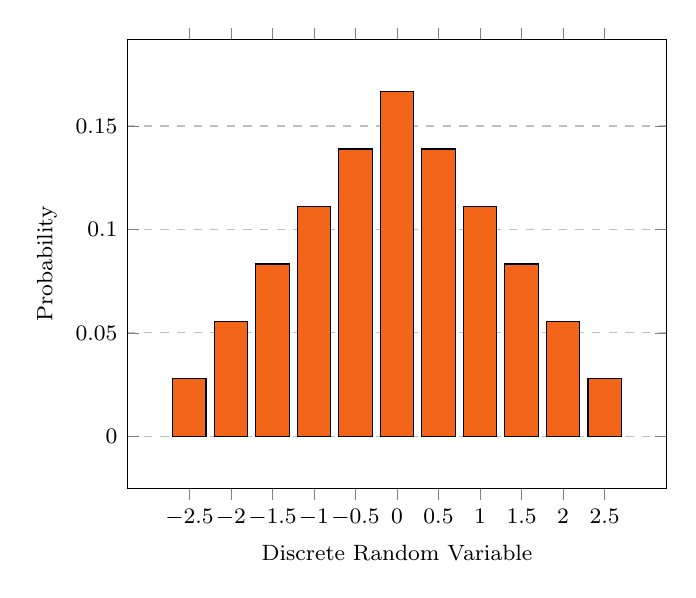
\begin{tikzpicture}
    \begin{axis}[
        ybar,
        bar width=12pt,
        ymin=0,
        xlabel={Discrete Random Variable},
        ylabel={Probability},
        xtick={-2.5,-2,...,2.5},
        xticklabel style={font=\footnotesize},
        yticklabel style={font=\footnotesize, /pgf/number format/fixed},
        xlabel style={font=\footnotesize},
        ylabel style={font=\footnotesize},
        xticklabel style={/pgf/number format/fixed},
        enlargelimits=0.15,
        ymajorgrids=true,
        grid style=dashed
    ]
    \addplot[fill={rgb,255:red,243;green,102;blue,25}] coordinates {
        (-2.5, 0.0278)
        (-2.0, 0.0556)
        (-1.5, 0.0833)
        (-1.0, 0.1111)
        (-0.5, 0.1389)
        (0.0, 0.1667)
        (0.5, 0.1389)
        (1.0, 0.1111)
        (1.5, 0.0833)
        (2.0, 0.0556)
        (2.5, 0.0278)
    };
    \end{axis}
\end{tikzpicture}
\caption{\label{fig:law_large_numbers_1}Probability mass function of the discrete random variable $\frac{X_1 + X_2 }{2} - \mathbb{E}(X)$.}
\end{figure}

Now let's consider a random sample of size ten. In Figure \ref{fig:law_large_numbers_2} is depicted the probability mass function of the discrete random variable $\frac{X_1 + X_2 + \ldots +  X_{10}}{10} - E(X): \Omega \times \ldots \times \Omega \rightarrow \mathbb{R}$. The probability $P(  |\frac{X_1 + X_2 + \ldots +  X_{10}}{10} - E(X)| < 1 )$ is $0.973$.

\begin{figure}[t]
\centering
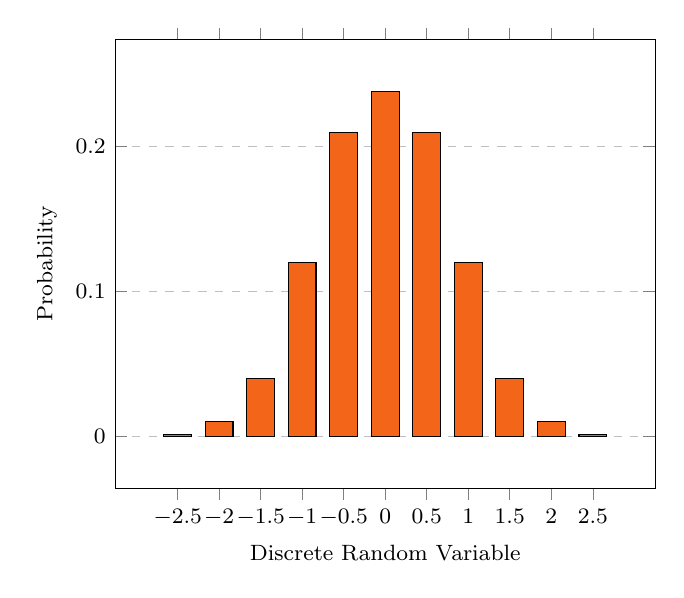
\begin{tikzpicture}
    \begin{axis}[
        ybar,
        bar width=10pt,
        ymin=0,
        xlabel={Discrete Random Variable},
        ylabel={Probability},
        xtick={-2.5,-2,-1.5,-1,-0.5,0,0.5,1,1.5,2,2.5},
        xticklabel style={font=\footnotesize},
        yticklabel style={font=\footnotesize},
        xlabel style={font=\footnotesize},
        ylabel style={font=\footnotesize},
        xticklabel style={/pgf/number format/fixed},
        enlargelimits=0.15,
        ymajorgrids=true,
        grid style=dashed
    ]
    \addplot[fill={rgb,255:red,243;green,102;blue,25}] coordinates {
        (-2.5, 0.0010)
        (-2.0, 0.0100)
        (-1.5, 0.0400)
        (-1.0, 0.1200)
        (-0.5, 0.2100)
        (0.0, 0.2380)
        (0.5, 0.2100)
        (1.0, 0.1200)
        (1.5, 0.0400)
        (2.0, 0.0100)
        (2.5, 0.0010)
    };
    \end{axis}
\end{tikzpicture}
\caption{\label{fig:law_large_numbers_2}Probability mass function of the discrete random variable $\frac{X_1 + X_2 + \ldots +  X_{10}}{10} - E(X)$.}
\end{figure}

\end{example}

It is important to clarify that the law of large numbers refers to the sample mean, that is $\frac {1}{n} \sum_{i=1}^{n} X_{i}$, and it is not necesarily true for other formulas, like for example, the deviation from the theoretical expected value $\sum_{i=1}^{n} X_{i} - n \times E(X)$ which not only it does not converge, but inscreases in absolute value as $n$ increases (see Example \ref{ex:gambler's_fallacy}).

\begin{example}
\label{ex:gambler's_fallacy}
If we toss a fair coin, the probability that the outcome will be head is equal to $1/2$. According to the law of large numbers, the proportion of heads in a large number of coin tosses will be close to $1/2$. However, the difference between the number of heads and tails will not be close to zero. In fact, the larger the number of coin tosses, the larger will be this difference. This is a highly conterintuitive fact, since most of the people think that the more we toss the coin, the closer will be the number of heads to the number of tails, which is not true.
\end{example}

% Central Limit Theorem

\subsection{Central Limit Theorem}

Let $X_1, \ldots, X_n$ be a sample of $n$ independent and identically distributed discrete random variables with mean $\mu$ and variance $\sigma^2$. As we saw in the previous section, the law of large numbers states that the sample average $\overline {X}_n$ converges in probability to $\mu$ as $n$ increases. The central limit theorem states that the distribution of the difference between the sample average $\overline {X}_n$ and the population mean $\mu$, when multiplied by the factor $\sqrt {n}$ approximates to the normal distribution with mean $0$ and variance $\sigma^2 / n$. The theorem is true regardless of the shape of the original random vairables.

\begin{theorem}[Central Limit Theorem]
\label{th:central_limit_theorem_pdf}\index{Central limit theorem}
Let $X_{1}, \ldots, X_{n}$ be a random sample of size $n$ from a distribution with mean $\mu$ and finite variance $\sigma^{2}$. Define the standardized sum as
\[
Z_n = \frac{\overline{X}_{n}-\mu}{\sigma/\sqrt{n}},
\]
where $\overline{X}_{n} = \frac{1}{n} \sum_{i=1}^{n} X_i$ is the sample mean. Then, as $n \rightarrow \infty$, the probability density function of $Z_n$ converges to the probability density function of the standard normal distribution $\phi(x)$, that is,
\[
\lim_{n \rightarrow \infty} f_{Z_n}(x) = \phi(x),
\]
where $f_{Z_n}(x)$ is the probability density function of $Z_n$, and $\phi(x)$ is the probability density function of the standard normal distribution, given by
\[
\phi(x) = \frac{1}{\sqrt{2\pi}} \exp\left(-\frac{x^2}{2}\right).
\]
\end{theorem}
\begin{proof}
Let $X_{1}, \ldots, X_{n}$ be independent and identically distributed (i.i.d.) discrete random variables with mean $\mu$ and finite variance $\sigma^2$. Define the sample mean as
\[
\overline{X}_n = \frac{1}{n} \sum_{i=1}^{n} X_i.
\]
We are interested in the distribution of the standardized variable
\[
Z_n = \frac{\overline{X}_n - \mu}{\sigma / \sqrt{n}}.
\]

First, consider the sum of the $X_i$'s, which we write as
\[
S_n = \sum_{i=1}^{n} X_i.
\]
The sample mean can then be written as
\[
\overline{X}_n = \frac{S_n}{n}.
\]
Thus, the standardized variable $Z_n$ becomes
\[
Z_n = \frac{S_n - n\mu}{\sigma\sqrt{n}}.
\]

To analyze the behavior of $Z_n$ as $n \to \infty$, we consider the sum $S_n = \sum_{i=1}^{n} X_i$. According to the Law of Large Numbers, $S_n/n$ converges to $\mu$, and hence $Z_n$ should converge to a normal distribution due to the nature of sums of independent discrete random variables.

For large $n$, $Z_n$ can be approximated by considering the Taylor expansion of the exponential function. Since the $X_i$'s are i.i.d., the distribution of $S_n$ can be approximated by a normal distribution with mean $n\mu$ and variance $n\sigma^2$. The key idea is that as $n$ increases, the distribution of $Z_n$ approaches a normal distribution because the sum of i.i.d. discrete random variables tends to be normally distributed by the Central Limit Theorem.

Let us consider the moment generating function (MGF) of $Z_n$. The MGF of $Z_n$ is given by:
\[
M_{Z_n}(t) = \mathbb{E}\left[\exp\left(t Z_n\right)\right] = \mathbb{E}\left[\exp\left(t \frac{S_n - n\mu}{\sigma\sqrt{n}}\right)\right].
\]
For large $n$, by the Central Limit Theorem, the MGF of $Z_n$ approaches that of a standard normal variable $N(0,1)$:
\[
M_{Z_n}(t) \approx \exp\left(\frac{t^2}{2}\right),
\]
which implies that $Z_n$ converges in distribution to $N(0,1)$ as $n \to \infty$.

Since $Z_n$ converges in distribution to $N(0,1)$, the probability density function of $Z_n$, denoted by $f_{Z_n}(x)$, must converge to the probability density function of a standard normal distribution $\phi(x)$, given by:
\[
\phi(x) = \frac{1}{\sqrt{2\pi}} \exp\left(-\frac{x^2}{2}\right).
\]
Thus, we have
\[
\lim_{n \rightarrow \infty} f_{Z_n}(x) = \phi(x).
\]

Therefore, as $n \to \infty$, the distribution of the standardized sum $Z_n$ approaches the standard normal distribution, completing the proof.
\end{proof}

The Central Limit Theorem is a fundamental concept in probability theory used in statistical analysis and inference. It allows us to compute the probability that the sample average is close to the distribution mean. It is important to recall the conditons for the central limit theorem to be true: the samples must be independent and identically distributed, the original distribution has to have a finite variance, and the sample size must be sufficiently large.

\begin{example}
Suppose a factory produces light bulbs, and the lifespan of each light bulb is a discrete random variable with a mean of $\mu = 1000$ hours and a standard deviation of $\sigma = 50$ hours. The factory tests a random sample of $n = 36$ light bulbs to estimate the average lifespan of the bulbs produced in a particular batch. What is the probability that the sample mean lifespan of these 36 bulbs is between 990 and 1010 hours?

We can apply the Central Limit Theorem to solve this problem because we are dealing with the sample mean of a large number of independent, identically distributed discrete random variables (lifespans of light bulbs). First, define the sample mean $\overline{X}_n$ as:
\[
\overline{X}_n = \frac{1}{n} \sum_{i=1}^{n} X_i,
\]
where $X_i$ represents the lifespan of the $i$-th light bulb in the sample, and $n = 36$ is the sample size.

By the Central Limit Theorem, for sufficiently large $n$, the distribution of the sample mean $\overline{X}_n$ approaches a normal distribution with mean $\mu$ and standard deviation $\sigma/\sqrt{n}$:
\[
\overline{X}_n \sim N\left(\mu, \frac{\sigma}{\sqrt{n}}\right) = N\left(1000, \frac{50}{\sqrt{36}}\right) = N\left(1000, \frac{50}{6}\right) = N\left(1000, 8.33\right).
\]

Next, we calculate the z-scores corresponding to 990 hours and 1010 hours using the formula:
\[
z = \frac{X - \mu}{\sigma/\sqrt{n}},
\]
where $X$ is the value for which we want to find the z-score.

For $X = 990$:
\[
z_{990} = \frac{990 - 1000}{8.33} \approx \frac{-10}{8.33} \approx -1.20.
\]

For $X = 1010$:
\[
z_{1010} = \frac{1010 - 1000}{8.33} \approx \frac{10}{8.33} \approx 1.20.
\]

Now, we use the standard normal distribution table (or a calculator) to find the probabilities corresponding to these z-scores:
\[
P(z_{990} \leq Z \leq z_{1010}) = P(-1.20 \leq Z \leq 1.20).
\]

From the standard normal distribution table:
\[
P(Z \leq 1.20) \approx 0.8849,
\]
\[
P(Z \leq -1.20) \approx 0.1151.
\]

Thus, the probability that the sample mean lifespan of the 36 light bulbs is between 990 and 1010 hours is:
\[
P(990 \leq \overline{X}_n \leq 1010) = P(-1.20 \leq Z \leq 1.20) = 0.8849 - 0.1151 = 0.7698.
\]

The probability that the sample mean lifespan of the 36 light bulbs falls between 990 and 1010 hours is approximately 76.98\%. This result demonstrates how the Central Limit Theorem allows us to use the normal distribution to approximate the sampling distribution of the sample mean, even when the original data is not normally distributed, as long as the sample size is sufficiently large.
\end{example}

%
% Section: References
%
\section*{References}

\cite{degroot1986probability} is a widely respected textbook in the fields of statistics and probability theory. First published in 1975, this book is known for its clear exposition of the fundamental concepts of probability and statistics, making it suitable for both beginners and those with some background in the subject. The book's approach balances theory and application, making it useful both for learning theoretical underpinnings and for applying probability and statistics to real-world problems.

\cite{childers2013philosophy} offers a comprehensive introduction to the foundational aspects of probability, with a focus on the philosophical questions it raises. Childers explores various interpretations of probability, including frequentist, propensity, classical, Bayesian, and objective Bayesian, and presents these complex ideas in a way that is accessible even to those without a strong background in probability or mathematics.

An example of the problems associated with the misinterpretation of expected value is the St. Petersburg Paradox\index{St. Petersburg Paradox}. Introduced by Nicholas Bernoulli in 1713, this paradox involves a gambling game with an infinite expected payoff, yet no reasonable person would pay more than \$25 to play it. Despite being three centuries old, the paradox continues to inspire new arguments and solutions in recent years (see \cite{huang2013three} for a historical review of the main proposed solutions).
